%----------------------------------------------------------------
% FEUILLE DE STYLE ENSG au format Latex
% Création : sept. 2010 (D Lercier)
% Modification sept. 2012 (T Coupin)
%----------------------------------------------------------------

\documentclass{themeensg}

%---Texte en filigranne---
%pour l'enlever : \SetWatermarkText{}
%-------------------------

%---Mes packages à moi---
%\usepackage{}
%------------------------

%---Mes raccourcis---
\newcommand{\transpose}[1]{{}^t \! #1}
\newcommand{\ensg}{\textsc{Ensg}}
%--------------------

%---Paramètres du pdf---
    \hypersetup{
       backref=true,                           % Permet d'ajouter des liens dans
       pagebackref=true,                       % les bibliographies
       hyperindex=true,                        % Ajoute des liens dans les index.
       colorlinks=true,  %Colorise les liens : true pour version numérique, false pour version d'impression
       breaklinks=true,                        % Permet le retour à la ligne dans les liens trop longs.
       urlcolor= blue,                         % Couleur des hyperliens.
       linkcolor= blue,                       % Couleur des liens internes.
       bookmarks=true,                         % Créé des signets pour Acrobat.
       %bookmarksopen=true,                    % Si les signets Acrobat sont créés,
                                               % les afficher complètement.
       pdftitle={Thème ENSG},                 % Titre du document.
                                               % Informations apparaissant dans
       pdfauthor={Mohamed-Amjad LASRI},                      % dans les informations du document
       pdfsubject={rapport de TFE}           % sous Acrobat.
    }

%-----------------------



%-------------------------------------------------------------

\setcounter{tocdepth}{1} %profondeur de la table des matières

\title{Intégration d’un dispositif de communication  en champ proche (NFC) au geocube\\Version provisoire du \today~à \timenow}

%
%-------------------------------------------------------------
% Début du document
%--------------------------------------------------------------
\begin{document}
%--------------------------------------------------------------
\begin{titlepage}
%Inclusion des labels des entreprises
%Pour un seul label (à gauche), mettre NULL pour les 3e et 4e argument
\enterprise 
{logos/IGN_logo.png}
{}
{logos/kylia_logo.png}
{}

%Inclusion du titre
\maketitle{Stage de fin d'études \\Cycle des Ingénieurs diplômés de l'ENSG 3\up{ème} année }{images/geogeo.png}

\infos{Mohamed-Amjad LASRI}{Septembre 2015}
\end{titlepage}


%---Page du jury---
%---Page du jury---
\newevenpage
\thispagestyle{plain}
\section*{Jury}
\vspace{0.5cm}

\textbf{Président de jury :} \\

Pierre-Yves Hardouin, directeur des enseignements de l'ENSG

\vspace{0.5cm}

\textbf{Commanditaire :} \\

KYLIA


Laboratoire d’Opto-Electronique, Métrologie et Instrumentation (LOEMI), Institut de l’Information Géographique et Forestière (IGN)

\vspace{0.5cm}

\textbf{Encadrement de stage :} \\ 

Olivier Martin IGN/DRE/SRSIG/LOEMI

Frédéric Verluise KYLIA

Emmanuel Bardière ENSG

\vspace{0.5cm}

\textbf{Responsable pédagogique du cycle Ingénieur :} \\

Serge Botton, IGN/ENSG/DE/DPTS

\vspace{0.5cm}

\textbf{Tuteur du stage pluridisciplinaire :} \\

Patricia Parisi, IGN/ENSG/DE/DSHI

\vspace{1cm}

\copyright \hspace{0.3cm} ENSG

\section*{Stage de fin d'étude du 04/05/2015 au 04/10/2015 }
\vspace{0.3cm}
\textbf{Diffusion web :} $\boxtimes$ Internet \hspace{0.2cm}$\boxtimes$ Intranet Polytechnicum\hspace{0.2cm}
$\boxtimes$ Intranet ENSG\vspace{0.3cm}

\textbf{Situation du document :} 
\vspace{0.2cm}
\par
Rapport de stage de fin d'études présenté en fin de 3\up{ème} année du cycle des Ingénieurs
\vspace{0.3cm}


\newcounter{x}
\setcounter{x}{\getpagerefnumber{LastPage}-\getpagerefnumber{beginappendices}+1}

\textbf{Nombres de pages :} 50 pages dont 3 d'annexes
\vspace{0.3cm}

\textbf{Système hôte :} \LaTeX
\vspace{1cm}


\textbf{Modifications :} 
\begin{center}
\begin{tabular}{|c|c|c|>{\centering}p{6.5cm}|}
\hline 
EDITION & REVISION & DATE & PAGES MODIFIEES\tabularnewline
\hline
\hline 
1 & 0 & 09/2015 & Création\tabularnewline
\hline 

\end{tabular}
\end{center}
%------------------

%------------------------------------------------------------------------------
% Remerciements
%\newevenpage
\chapter*{Remerciements}

Je tiens à remercier toutes les personnes qui ont participé de différentes façons à la réussite de mon stage et plus particulièrement les personnes que je cite ci-dessous.

Olivier MARTIN, Frederic VERLUISE, Christian THOM et Christophe MEYNARD qui m'ont encadré, conseillé et ont répondu régulièrement à mes questions tout au long de mon stage.

Emmanuel BARDIERE, mon référent de stage ENSG, qui a suivi l'évolution de mon stage tout au long de ces cinq mois.

Tout le personnel du Laboratoire d'Opto-Électronique de Metrologie et d'Instrumentation de l'Institut National de l'Information Géographique et Forestière et de la société KYLIA.


%---Résumé (français)---
\begin{abstract}
\thispagestyle{empty}
	\vspace{1cm}

	Dans ce rapport, je présente le travail effectué lors de mon stage de fin d'études: une implémentation du protocole de transfert des blocs de l'ISO/IEC 14443-4 realtif aux puces NFC dans le système d'exploitation du Géocube G3OS, en plus du développement d'une antenne et de l'interface Android dédiée. A cela s'ajoute la conception, le développement et le déploiement d'un système de mises à jour du coordinateur des Géocubes, et la mise en place partielle d'une pipeline de production des logicielles au sein de la société Kylia.
	
	\vspace{1.5cm}
	
	\textbf{Mots clés :} NFC, systèmes embarqués, production des logicielles,
\end{abstract}
%-----------------------


%---Résumé (anglais)---
\selectlanguage{english}
\begin{abstract}
\thispagestyle{empty}
	\vspace{1cm}
	
	I present the work done during my internship graduation: an implementation of the Block Transfert Protocol of the Near Field Communication (NFC) standard ISO / IEC 14443-4 in the Géocube's operating system G3OS, in addition to developing an  NFC antenna and an Android dedicated GUI. Added to this is the design, development and deployment of an updating system  Géocubes coordinator, and the partial implementation of a software production pipeline within the company Kylia.
	
	\vspace{1.5cm}
	
	\textbf{Key words:}  NFC, embedded systems, software production,
\end{abstract}
%----------------------

\selectlanguage{frenchb}

%---Table des matières, des figures et des tableaux---
%\newevenpage
\tableofcontents

\newevenpage
\listoffigures

\newevenpage
\listoftables
%----------------------------------------------------

%\newevenpage
\chapter*{Glossaire et sigles utiles}
\addcontentsline{toc}{chapter}{Glossaire et sigles utiles}

  \begin{acronym}
  \acro{ENSG}{\'Ecole Nationale des Sciences Géographiques}
  \acro{FIFO}{First In First Out}
  \acro{G3OS}{Geocube Operating System}
  \acro{GNSS}{Global Navigation Satellite Systems}
  \acro{GPS}{Global Positionning System}
  \acro{IEC}{The International Electrotechnical Commission}
  \acro{IHM}{Interface Homme Machine}
  \acro{ISO}{The International Organization for Standardization}
  \acro{NFC}{Near Field Communication}
  \acro{PCD}{Proximity Coupling Device}
  \acro{PICC}{Proximity Inductive Coupling Card}
  \acro{RTOS}{Real Time Operating System}
  \acro{TCP/IP}{Transmission Control Protocol/Internet Protocol}
  \end{acronym}


%---Introduction------------------------------------------------------------------
\newevenpage
\chapter*{Introduction}
  \addcontentsline{toc}{chapter}{Introduction}
  
  \vspace{1.5cm}
  
	Les objets connectés sont de plus en plus présents dans notre quotidien: Nos cartes bancaires, nos cartes de transports, nos smartphones, les arrêts de bus, etc, sont tous équipés de puces NFC. Cette technologie, utilisée généralement pour partager des identifiants ou des informations peu volumineuse se voit démocratisée et normée, offrant au concepteur des produits novateurs une solution de communication simple et à la disposition du large publique.
	
	L'objectif de ce stage est d'intégrer une solution de communication en champ proche (NFC) au Géocube. Ceci sous entend le développement les couches matérielles et logicielles de cette solution, ainsi qu'une application Android dédiée. En plus du sujet principal du stage deux autres tâches relatives à la mise en place d'un serveur de production des logiciels et un système de mise à jour automatique du coordinateur des Géocubes ont été réalisées.
	
	Dans le premier chapitre de ce rapport, on présente les notions fondamentales nécessaires au lecteur pour comprendre le travail effectué. Le contenu de ce rapport touche à plusieurs disciplines (électronique, systèmes embarqués, réseaux, sécurité informatique, ...) la lecture du premier chapitre est fortement conseillée. Le deuxième chapitre résume la conception et le développement relatif à la solution NFC implémentée dans le Géocube, on présente les expérimentations électroniques réalisées pour choisir une antenne NFC adaptée au Géocube, les développements effectués sur G3OS\footnote{Système d'exploitation du Géocube} pour implémenter le 4ème niveau de la norme ISO14443 relative au protocole de transmission des blocs NFC et finalement le développement de l'application Android dédiée. Dans le 3ème chapitre, On présente le travail effectué pour concevoir, développer et déployer une solution de mises à jour automatique pour le coordinateur des Géocubes. Finalement, le 4ème chapitre donne un aperçu sur l'infrastructure virtuelle de production des logiciels instaurée pour répondre au besoin de la société Kylia de disposer d'un serveur de production adaptée à ses besoins.
	
	 On note ici que tous les codes produits durant ce stage restent la propriété des organismes d'accueil et ont la liberté de choisir la licence appropriée. pour toute demande de consultation de ces codes, le lecteur est prié de s'adresser directement aux encadrants.

%-------------------------------------------------------------------------------

\evenchapter[Concepts clés et problématiques]{Concepts clés et problématiques}

\textit{ Ce chapitre a pour but d'introduire le lecteur aux concepts clés nécessaires pour comprendre le travail effectué lors de ce stage.
Le lecteur est prié de prêter une attention particulière au tableau des sigles lors de la lecture du présent document. Les protocoles qu'on présente utilisent un certain nombre d’abréviations conventionnelles pour désigner Les opérations d'échanges entre les dispositifs, spécialement NFC. }

\section{Les Géocubes}
La miniaturisation des capteurs ainsi que la baisse des coûts de fabrication et de la consommation électrique des puces GNSS sont des facteurs qui peuvent laisser à envisager d'abandonner sur le terrain un réseau de capteurs opérant en permanence. Certains de ces capteurs GNSS permettent d'effectuer des mesures sur la phase donnant la possibilité de remonter à des précisions millimétriques, d'où l'idée d'un réseau de Géocubes. Le système Géocube est un réseau de capteurs GPS conçu et développé par le Laboratoire d'Opto-Éléctronique, Métrologie et Instrumentation de l'Institut National de l'Information Géographique et Forestière. Il a comme objectif de mesurer les déformations avec une précision millimétrique. Ce réseau de capteurs a la particularité d'être très peu gourmand en énergie. On peut envisager de l'abandonner dans un milieu difficilement accessible sans qu'on ait à se soucier de son alimentation continue en électricité. En plus d'un module radio, un Géocube peut supporter plusieurs couches de capteurs lui permettant de collecter un certain nombre d'informations sur son environnement.

Dans les premières versions du Géocube initiés par LOEMI, Un opérateur humain peut communiquer directement avec un géocube en utilisant une de ces méthodes:

\begin{itemize}
\item Liaison série filaire, qui permet d'envoyer des commandes  à travers l'interface en lignes de commandes de G3OS.
\item Radio: Un protocol propriétaire particulier (DigiMesh\textcopyright) est utilisé pour communiquer avec un Géocube.
\end{itemize}

Dans la version industrielle du Géocube maintenue par la société Kylia, une attention particulière est prêtée à l'étanchéité du boîtier qui le contient et à la robustesse du produit final. Ce choix crucial se justifie principalement par le fait qu'un réseau de Géocube peut être destiné à la surveillance environnementale en temps de crise et doit, par conséquence, être résistant aux conditions extremes que peut présenter un tel contexte.

Un réseau de Géocubes communique à travers le protocole radio DigiMesh\textcopyright et l'utilise aussi pour centraliser les mesures acquises par les Géocubes vers un ordinateur déployé aussi sur le terrain, appelé coordinateur. Le coordinateur est le composant central du réseau, il encapsule toute la logique liée au traitement et au stockage des données. Il permet aussi à l'utilisateur de lancer des séries de calculs, récupérer les résultats ou de communiquer avec un Géocube en lançant des commandes qui seront transmises par radio. La Figure\ref{fig:geocube_network} résume ce schéma de fonctionnement.

\begin{figure}[h!]
\centering
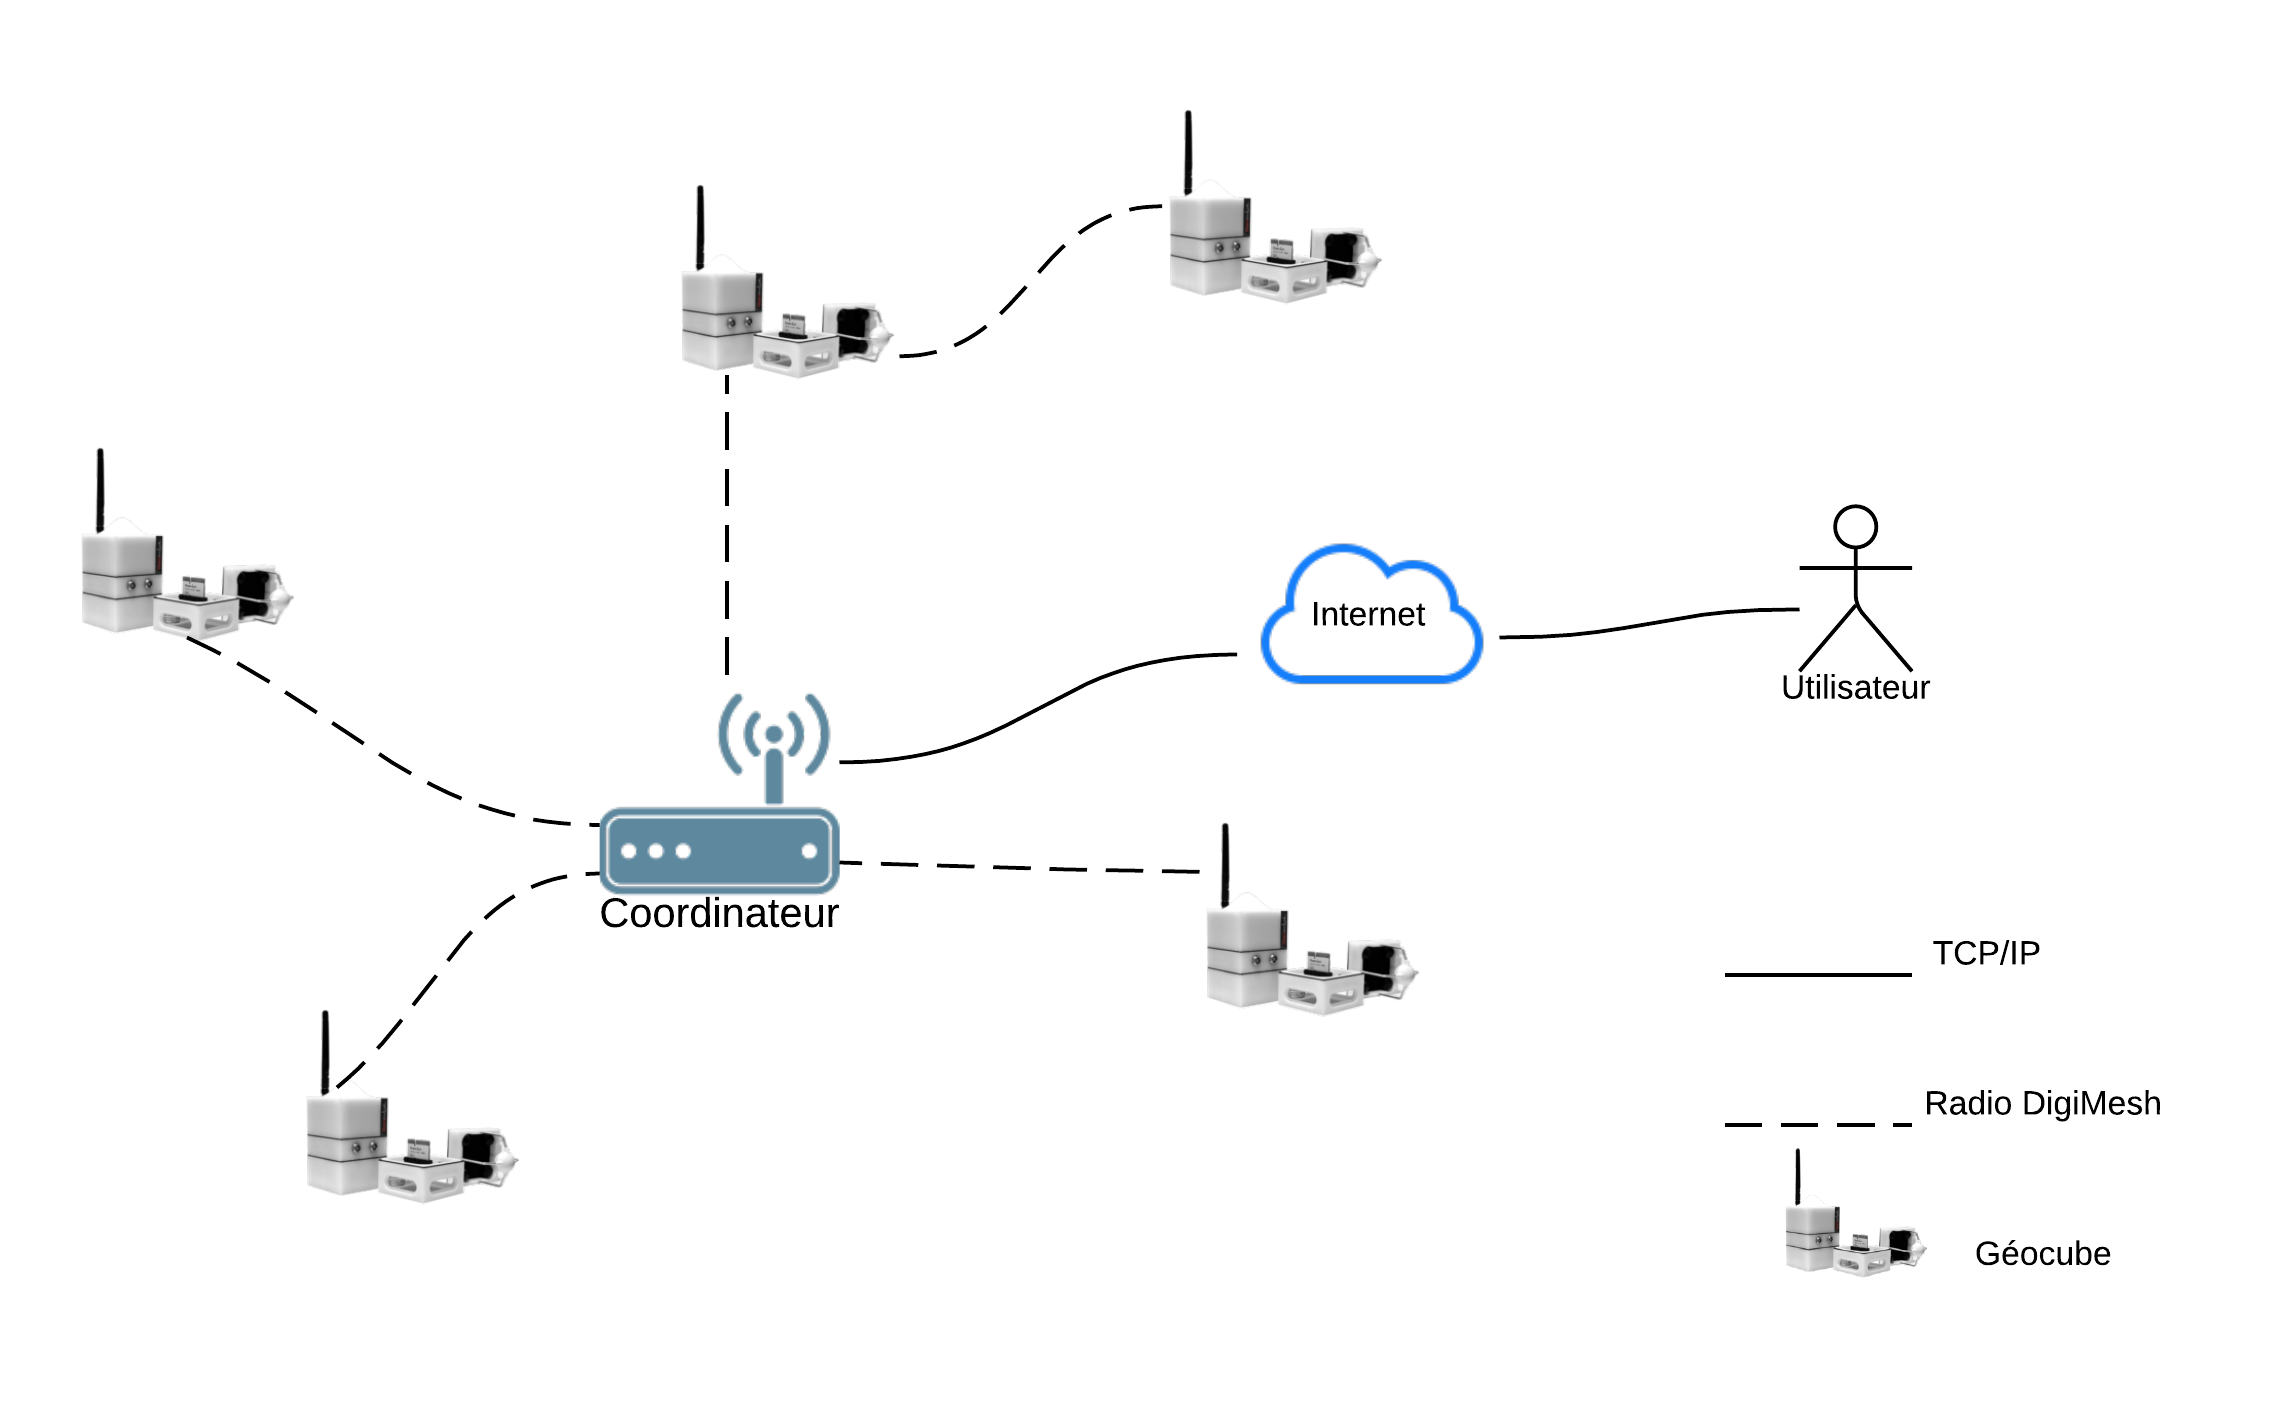
\includegraphics[scale=0.8]{images/fig1.png}
\caption{Un réseau de Géocubes}
\label{fig:geocube_network}
\end{figure}

\section{Les systèmes embarqués et les noyaux temps-réel dur:}
Un système embarqué est par définition: Un système éléctronique et informatique autonome, souvent temps-réel, spécialisé dans une tâche bien précise [1]. De cette définition on peut ressortir deux éléments clés:
\begin{itemize}
\item Un système embarqué nécessite un développement matériel (électronique) mais aussi logiciel.
\item Un système embarqué a la particularité d'opérer en temps-réel.
\end{itemize}
Le lecteur peut se poser la question légitime: Pourquoi on insiste sur le "temps-réel" dans cette définition? Nos ordinateurs personnels n'opèrent-ils pas en "temps-réel"?. Pour répondre à ces questions et introduire l'importance du temps-réel dans le cas du système Géocube Il faut comprendre que ce concept est très relatif en informatique et varie d'un métier à un autre: Le temps-réel pour un développeur web est de pouvoir fournir à l'internaute de l'information sous forme de flux, en tolérant les temps de latence qui peuvent résulter parfois des temps d'accès à une base de données ou à la bande passante d'internet. Pour un développeur qui fait de l'informatique pour automobiles et doit, par exemple, développer les couches logicielles relatives à un système d'airbag, Le temps-réel dans ce cas est très strict et la quantification de ce temps latence est primordiale, sinon la vie des gens serait en danger.
\subsection{Les tâches}
Une tâche est le composant principal d'un RTOS. Lorsque vous effectuez plusieurs tâches simultanées sur un ordinateur avec une mémoire vive limitée, vous pouvez remarquer à partir d'un certain ... que vos tâches auront du mal à tourner ... Pour les systèmes d'exploitation en temps-réel, communément connus sous le nom de RTOS (Real Time Operating Systems) La quantification de ce temps de latence est primordiale.

Dans cette perspective, une équipe de chercheurs du LOEMI ont mis au point un RTOS adapté aux tâches qui sont effectuées par un Géocube.

Une liste non exhaustive de ces tâches serait alors:

\begin{itemize}
\item Une tâche GPS qui gère toutes les opérations en relation avec l'acquisition des données GPS:
\item Une tâche Radio qui gère toutes les orpérations relatives à l'envoi et  à la réception des données et des commandes par radio;
\item Une tâche accéléromètre qui gère l'acquisition des données de l'accéleromètre...
\end{itemize}

On note ici qu'à chaque tâche on affecte une priorité. On revient à notre exemple d'airbag pour mieux appréhender cette notion. Imaginons maintenant que dans un RTOS destiné à l'industrie automobile on ne donne pas à la tâche qui gère l'airbag la plus haute priorité. Cela reviendrait à dire qu'à 

\subsection{La communication entre les tâches}

Dans un RTOS généralement, et dans G3OS plus particulièrement, une tâche peut communiquer avec ses semblables ou répondre à des signaux provenant des capteurs, qu'on appelle interruption.

Un signal d'interruption permet à un composant du système embarqué de notifier le micro-contrôleur central de l'arrivée d'un événement qui mérite son attention. Le choix de ces événements se fait souvent en programmant les registres des composants du système. Conventionnellement, le registre qui permet de choisir les événements déclencheurs d'interruptions s'appelle le registre principal des interruptions (Main Interrupt Register).

La communication entre les tâches s'effectue par plusieurs méthodes. La principale connue est la queue de messages. Ce mécanisme permet à une tâche de communiquer avec les autres en envoyant des messages. Un exemple typique serait alors: une tâche qui s'occupe de l'acquisition des données d'une puce GPS. Dès qu'une nouvelle trame de données est disponible, Cette tâche envoie  et une autre du traitement de ces données, Dans ce cas la première tâche envoie à la deuxième les données acquises à travers la que

\begin{figure}[h!]
\centering
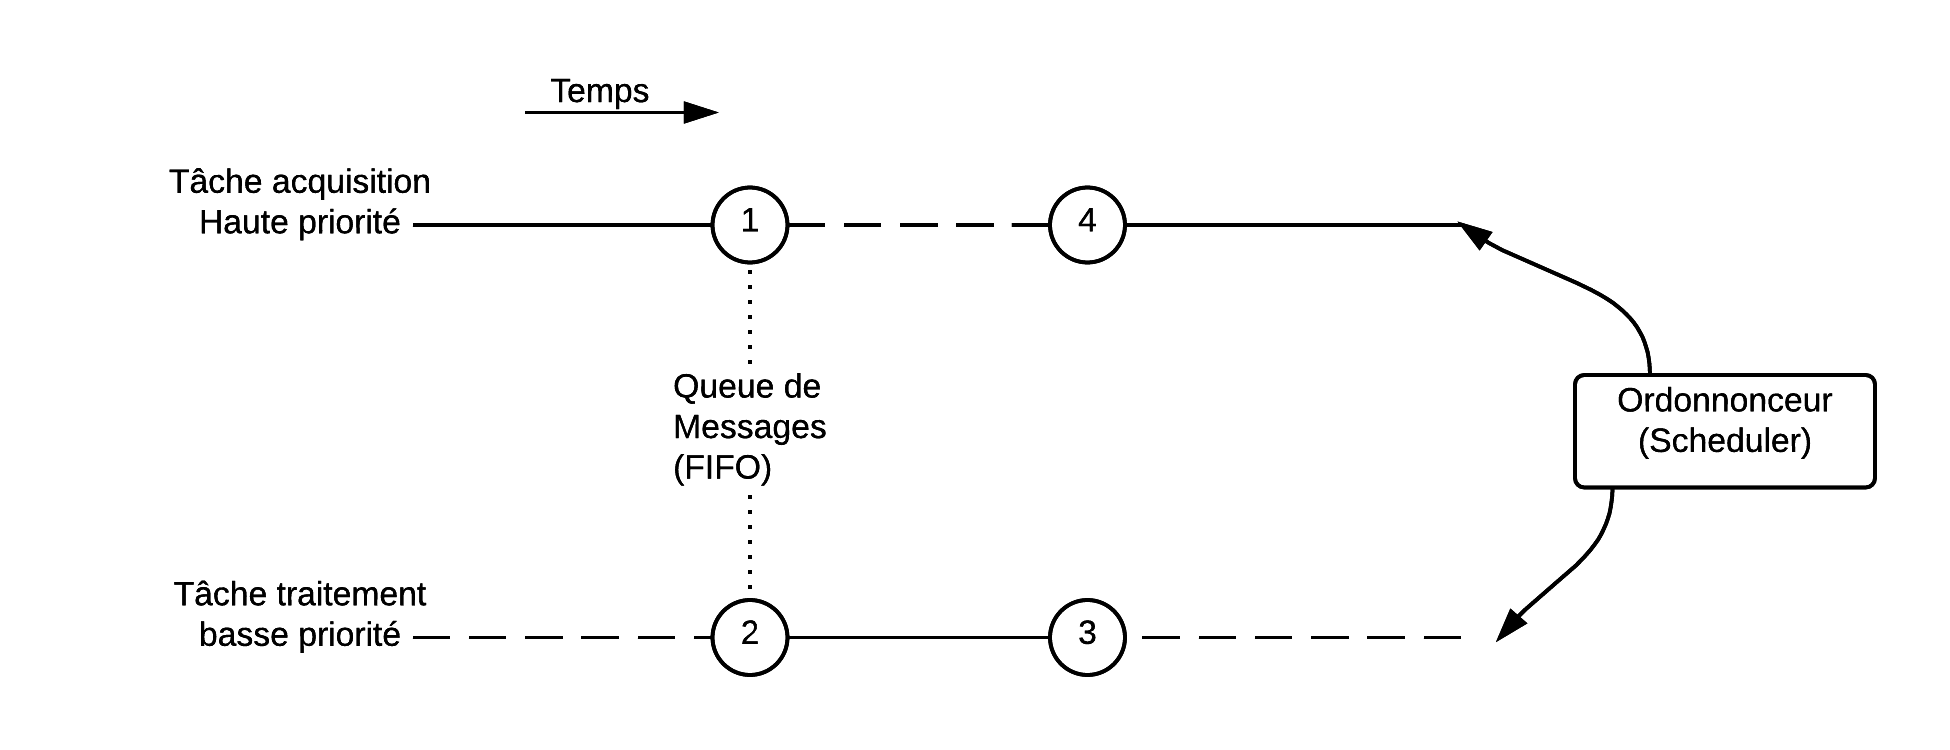
\includegraphics[scale=1]{images/fig2.png}
\caption{Exemple multi tâches}
\label{fig:multitask_ex}
\end{figure}

\section{La communication en champs proche (NFC)}
La communication en champs proche est un ensemble de protocoles permettant d'établir une connexion radio entre deux dispositifs avec une distance ne dépassant pas 4cm. Aujourd'hui, on compte des millions d'objets connectés contenant la technologie NFC(cartes bancaires, smartphone, arrêts de bus, smartwatch...). L'interopérabilité entre les différentes puces équipant ces objets a poussé les constructeurs à mettre en place un certain nombre de normes régissant la fabrication, la programmation et l'utilisation de cette technologie.

La guerre des normes a fait converger les constructeurs vers l'ISO/IEC 14443. Cette norme encapsule en elle même quatre sous normes:

\begin{itemize}
\item ISO/IEC 14443-1: Description des couches physiques
\item ISO/IEC 14443-2: 
\item ISO/IEC 14443-3:
\item ISO/IEC 14443-4: 
\end{itemize}

\subsection{couches matérielles:}
La conception des couches matérielles d'un circuit NFC doit respecter les recommandations de l'ISO/IEC 14443-1 et une partie de l'ISO/IEC 14443-2 pour garantir l'interopérabilité avec les autres dispositifs disponibles sur le marché. Un circuit NFC typique est composé de 3 parties principales:
\begin{itemize}
\item Une antenne: Selon les spécifications de la dite norme les dimensions de l'antenne ne doivent pas excéder 86mm x 54mm x 3mm.
\item Une capacité adaptée pour garantir une raisonnance du circuit sur la fréquence 13.56Mhz;
\item Le PICC
\end{itemize}
\subsection{couches logicielles:}


\section{Les infrastructures de production des logiciels}
La conception et le développement des solutions logiciels dans un milieu industriel nécessite des infrastructures permettant d'automatiser un certain nombre de tâches qui, ensemble, forment ce qui est communément connu sous le nom de pipeline de production logicielle.

Cette chaîne de production est itérative, Elle favorise les cycles courts pour délivrer au client un produit évolutif et s'adaptant à ses besoins. Dans la Figure... on présente les principales étapes de cette chaîne.

Comme montré dans la Figure.... Une pipeline de production logicielle a un certain nombre d'acteurs externes humains qui garantissent son alimentation en versions(1) et en tickets(2). On définit alors ces acteurs comme suit:

\begin{itemize}
\item Développeur: s'occupe de la conception et le développement des solutions informatiques en réponse aux besoins des clients exp.. dans le gestionnaire des bugs. Son travail permet d'alimenter le gestionnaire de versions.
\item Product owner: terme emprunté à la méthode Scrum. Il est l'interlocuteur unique des clients et permet de traduire leurs besoins en tickets(Gestionnaire de tickets)
\item Testeur: 
\end{itemize}
En plus de ces acteurs humains une infrastructure de production logicielle contient des composants logiciels pour automatiser un certain nombre de tâches:
\begin{itemize}
\item Gestionnaire de bugs: Comme son nom l'indique ce composant est un outil de communication et de traçabilité permettant de suivre l'évolution de la réponse du développeur au besoin du client et à la correction des bugs.
\item Gestionnaire de versions: Cet outil est un classique de la gestion des projets informatiques, il permet, entre autres, aux développeurs de collaborer sur le même code source sans que cela n'affecte  d'archiver tous les changements effectués sur un code source. Par souci de traçabilité, un gestionnaire de version est indispensable dans un projet informatique même s'il n y a qu'un développeur.
\item Intégration continue
\end{itemize}


\evenchapter[Conception et développement des couches logicielles et matérielles relatives à la norme NFC ISO14443 et de l'IHM Android dédiée]{Conception et développement des couches logicielles et matérielles relatives à la norme NFC ISO14443 et de l'IHM Android dédiée}

\section{Analyse du besoin:}
Dans le but de simplifier au maximum la mécanique et d’assurer au mieux l’étanchéité de celle-ci, il est prévu dans la version industrielle du geocube de n’utiliser ni interrupteur On/Off ni connecteur permettant de communiquer avec le geocube par un lien filaire. La seule possibilité de lien se fera par la radio, dont le débit est trop faible pour assurer des transfert de fichiers de données.

Solution :

Nous proposons donc d’inclure dans le geocube la fonctionnalité NFC. Elle devra pouvoir déclencher l’allumage ou au moins le réveil de sommeil profond du processeur du geocube, ainsi que son extinction. Elle devra aussi pouvoir servir de lien de communication avec le logiciel de commande du geocube pour permettre la configuration et le test de bon fonctionnement du geocube par exemple lors de son installation. Enfin, elle permettra le déchargement et le chargement de fichiers depuis et vers la carte µSD.
Le stage se déroulera en plusieurs phases :

- Identification du chipset NFC à utiliser. Il y en a un déjà dans le design actuel, il faudra vérifier si ses performances sont suffisantes.

- Modification ébventuelles de la carte du geocube pour intégrer le circuit choisi et assurer les fonctionnalités demandées.

- Test du chipset choisi.

- Réalisation des couches logicielles interface dans G3OS

- Réalisation d’une appli dédiée sous Android pour l’IHM


\subsection{Choix de la puce NFC:}
Le choix d'une puce NFC s'est basé sur une webographie effectuée sur les sites des constructeurs pour trouver la puce la plus adaptée à la description du besoin du commanditaire. Une puce NFC doit répondre au mieux à ce besoin tout en encapsulant le maximum de fonctionnalités des 3 derniers niveaux (2, 3 et 4) de la norme ISO-14443. Cette norme garantie l'interaction avec les dispositifs utilisant le système exploitation Android.

Après une première analyse des caractéristiques de quelques dix puces sélectionnées, On ne garde pour la suite que les trois citées dans le Tableau ci-dessous. La plupart des puces disponibles dans le marché et qui sont interfaçables avec un micro-contrôleur\footnote{La plupart des puces sont stand-alone et programmable une fois.}.
\begin{figure}
\begin{center}
\begin{tabular}{|c|c|c|c|c|c|c|c|}
\hline
Référence & Constructeur & Prix(\$) & Débit(kbps) & ISO 14443 & Interface & T° & RAM\\ \hline
TRF7970A & TI & 6.98 & 424 & 3 & SPI-Paral & -40°-110° & NC\\
RF430CL330H & TI & 1.74 & 848 & 3 & SPI-I2C & -40°-85° & 3KO\\
AS3953 & AMS & 1.09 & 848 & 3 & SPI & -40°-85° & NC\\
PN533 & NXP & NC & 848 & 3 & USB2 & -40°-125° & 1KO\\
\hline
\end{tabular}
\end{center}
\caption{Tableau comparatif des puces NFC présélectionnées.}
\end{figure}

On remarque qu'aucun constructeur ne propose des puces compatibles avec le 4ème niveau de la norme ISO/IEC 14443. L'utilisation de cette norme est indipensable pour pouvoir communiquer avec un dispositif Android\footnote{Android n'accepte pas les protocoles propriétaires pour la communication en champ proche. Que les protocoles certifiés par l'ISO/IEC}. Un travail serait alors à effectuer pour programmer le niveau manquant de la dite norme dans le micro-contrôleur.

Une puce existe déjà dans la version actuelle du Géocube. C'est l'AS3953, Le maintien de cette puce permettra de gagner:
\begin{itemize}
\item en temps de développement matériel.
\item en prix: c'est la moins cher de sa catégorie.
\item ultra basse consommation électrique\footnote{Ce qui est crucial pour le Géocube} Dans plusieurs cas d'utilisation la puce s'alimente de l'énergie émise par le smartphone.
\end{itemize}
Pour ces raison le choix de l'AS3953 a été maintenu pour le Géocube.

\section{Conception de la solution}

\subsection{Conception et expérimentation de l'antenne:}

Les prototypes des antennes NFC sont généralement conçus d'une manière empirique. Pour cela, Il existe plusieurs méthodes expérimentales conventionnelles. Mais avant de présenter les expériences réalisées. Il faut comprendre qu'un circuit NFC typique peut être assimilé à un circuit de type RLC. L'équivalent électrique d'une puce NFC et son antenne pourrait être assimilé au circuit de la Figure\ref{fig:nfcandantenna}.

\begin{figure}[h!]
\centering
\label{fig:nfcandantenna}
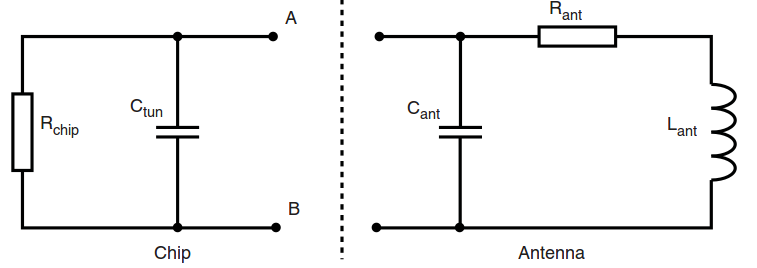
\includegraphics[scale=0.5]{images/chipANDantenna.png}
\caption{Circuit électrique équivalent d'une puce NFC et et son antenne}
\end{figure}
l'antenne est un fil conducteur, son équivalent électrique est la résistance $R_{ant}$. Elle a aussi une inductance qu'on note $L_{ant}$ et une capacité parasite $C_{ant}$. Alors que $R_{chip}$, $C_{tun}$ désignent respectivement la résistance et la capacité introduits par la puce NFC.

La Figure\ref{fig:nfcandantenna} est un schéma simplifié du circuit électronique que présente une antenne et une puce NFC puisqu'il ne prend pas en compte les connexions filaires entre les deux. Un schéma plus global peut se présenter comme dans la Figure\ref{fig:completeeq} lorsque l'antenne ajoute une résistance en série et dans la Figure\ref{fig:completeeq2} lorsque qu'elle inclut une résistance en parallèle.

\begin{figure}[h!]
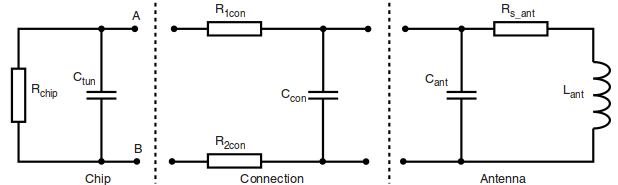
\includegraphics[scale=0.7]{images/chipANDantennaANDconn.png}
\label{fig:completeeq}
\caption{Circuit électrique équivalent d'une puce NFC, une antenne avec une résistance en série et les liaisons filaires entre les deux}
\end{figure}

\begin{figure}[h!]
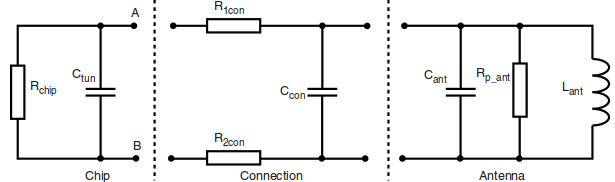
\includegraphics[scale=0.7]{images/withPARA.png}
\label{fig:completeeq2}
\caption{Circuit électrique équivalent d'une puce NFC, une antenne avec une résistance en parallèle et les liaisons filaires entre les deux}
\end{figure}
\begin{itemize}
\item $R_{con}$: La résistance équivalente parasite générée par les fils de connexion entre la puce NFC et l'antenne.
\item $C_{con}$: La capacité équivalente parasite générée par les fils de connexion entre la puce NFC et l'antenne.
\item $R_{s-ant}$: La résistance en série de l'antenne.
\item $R_{p-ant}$: La résistance en parallèle de l'antenne.
\end{itemize}
En calculant la résistance et la capacité équivalentes on obtient la Figure\ref{fig:circuiteq}. $R_{eq}$ est calculée comme suit:

\begin{figure}
\centering
\label{fig:circuiteq}
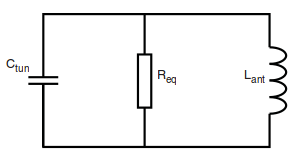
\includegraphics[scale=0.6]{images/circuiteq.png}
\caption{Circuit simplifié d'une puce NFC, une antenne et les connexions filaires entre les deux}
\end{figure}

$$R_{eq}=\frac{R_{chip}\times R_{p-ant}}{R_{chip}+R_{p-ant}}$$

alors que:

$$R_{p-ant}=R_{s-ant}\times(1+(\frac{L_{ant}\times\omega}{R_{s-ant}})^2)$$

La fréquence de raisonnance $f_0$ d'un circuit LC parallèle peut être calculée en utilisant cette formule:

$$f_0=\frac{1}{2\pi\sqrt{L_{ant}.C_{tun}}}$$

L'inductance de l'antenne à la raisonnance peut être exprimée comme suit:
$$L_{ant}=\frac{1}{(2\pi.f_0)^2.C_{tun}}$$

Dans la plupart des cas on dispose de l'inductance $L_{ant}$ dans les datasheets des antennes. La grandeur qui reste à déterminer est alors $C_{tun}$. Comme nous avons vu précédemment:

$$C_{tun}=C_{chip}+C_{conn}+C_{ant}$$

Les valeurs de $C_{ant}$ et $C_{chip}$ sont généralement disponibles dans les datasheets de l'antenne et de la puce NFC. Théoriquement, La seule grandeur qui reste à déterminer est $C_{conn}$:

$$C_{conn}=C_{tun}-C_{chip}-C_{ant}$$

Malheureusement, ce n'est pas toujours le cas\footnote{Comme c'est le cas pour le Géocube} le circuit imprimé sur lequel vient s'ajouter l'antenne NFC peut modifier l'inductance de l'antenne d'une manière (pseudo-)aléatoire et dépendante des composants rayonnants du circuit, en plus du plan de masse que peut présenter ce dernier. Un mode opératoire itératif qui consiste à faire varier la capacité $C_{conn}$ jusqu'à ce que la fréquence de raisonnance du circuit se stabilise autour de 13.56Mhz serait alors de.

Pour cela nous avons conçu l'expérimentation schématisée sur la Figure\ref{experience} Le but est alors de mesurer pour chaque itération(et donc pour chaque valeur de capacité) la fréquence de raisonnance du circuit à une antenne qui émet à 13.56Mhz\footnote{Ce qui simule l'antenne NFC d'un smartphone}, et ceci jusqu'à trouver la capacité pour laquelle le circuit: Géocube+antenne raisonne à 13.56Mhz. Un GBF(Générateur de Basses fréquences) réglé sur 13.56Mhz et lié à une antenne simule un smartphone avec son antenne NFC. Le but serait alors de mesurer à chaque itération, à l'aide d'un oscilloscope.

\begin{figure}[h!]
\centering
\label{experience}
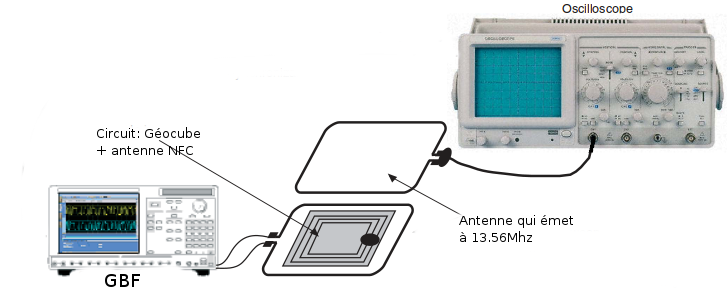
\includegraphics[scale=0.55]{images/gbfoscillo.png}
\caption{Expérimentation réalisée pour calibrer l'antenne NFC du Géocube}
\end{figure}
Les antennes testées sont des circuits éléctroniques imprimés que nous avons conçus spécialement pour le Géocube
Cette expérimentation a permit de choisir une capacité pour les modèles d'antennes....

\subsection{Conception statique des couches logicielles}
La puce NFC retenu n'inclut pas le niveau 4 de la norme ISO/IEC 14443. Ce niveau est indispensable pour pouvoir communiquer avec d'autres dispositifs NFC et spécialement les smartphones utilisant un système d'exploitation Android. Ce niveau contient les spécifications relatifs au protocole de transmission des données entre le PCD et le PICC qu'on nomme Le BTP(Block Transmission Protocol).

Le BTP définit un format de bloc tel montré dans le Tableau

\begin{tabular}[hf]{|c|c|c|c|c|c|c|c|}
\hline
\multicolumn{3}{|c|}{Prologue} & \multicolumn{3}{c|}{Information} & \multicolumn{2}{c|}{Epilogue} \\
\hline
PCB & [CID] & [NAD] & \multicolumn{3}{|c|}{[INF]} & \multicolumn{2}{c|}{EDC}\\
\hline
1 octet & 1 octet & 1 octet & \multicolumn{3}{|c|}{} & \multicolumn{2}{c|}{2 octets}\\
\hline
\end{tabular}

\subsubsection{Le prologue}
Le prologue contient les trois octets suivants:
\paragraph{PCB[obligatoire]:}
PCB (Protocol Control Byte)[obligatoire]: utilisé pour contrôler la transmission des données. Il peut être un de ces trois octets:
\begin{itemize}
\item I-Block Figure\ref{fig:I-Block} utilisé pour indiquer au dispositif destinataire que le bloc envoyé est un bloc d'information et contient des octets dans le champs INF.
\item R-Block Figure\ref{fig:R-Block} utilisé pour indiquer une reconnaissance négative ou positive. Un R-Block ne contient jamais de champs INF.
\item S-Block Figure\ref{fig:S-Block} utilisé pour échanger des informations de control entre le PCD et le PICC. Il existe deux types de S-Block: le DESELECT qui n'est jamais suivit par un champ INF et le WTE qui doit être suivit par un octets dans le champ INF.
\end{itemize}

\begin{figure}[h!]
\centering
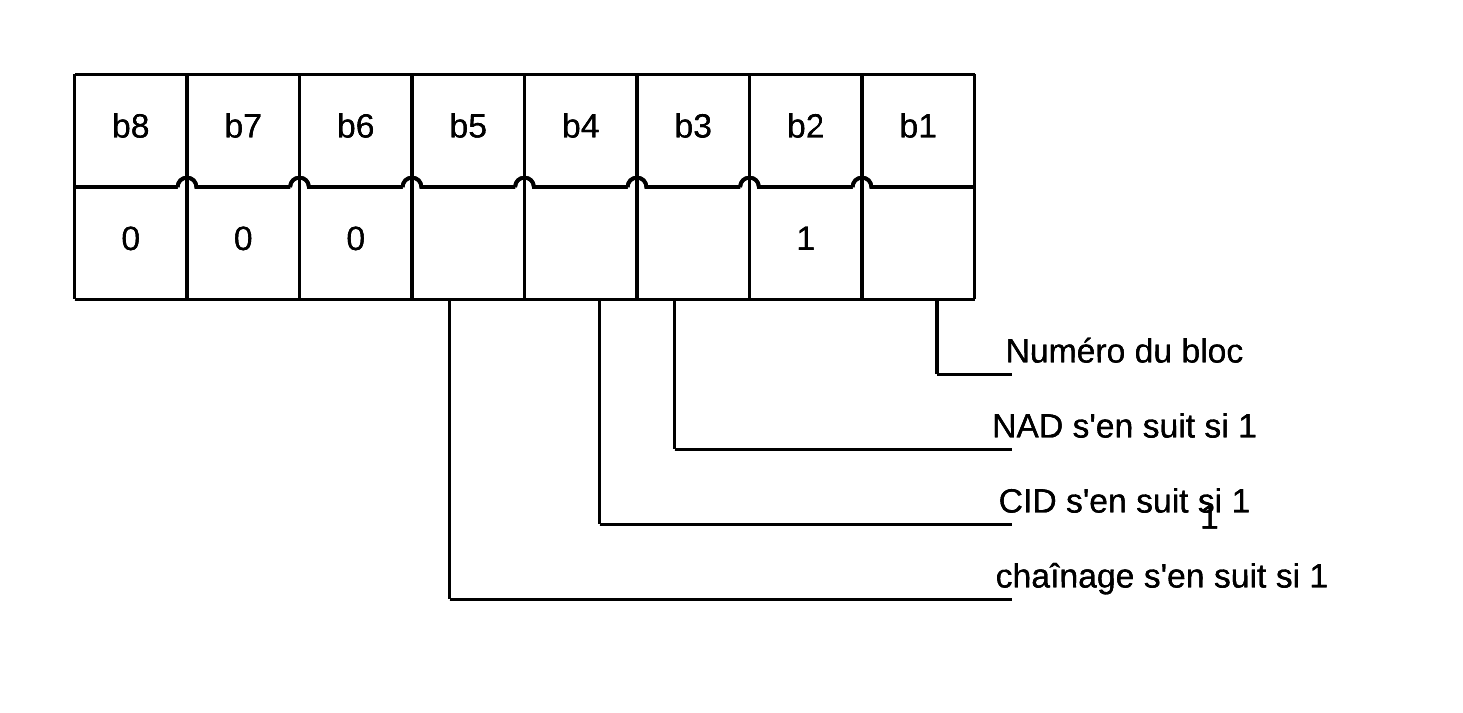
\includegraphics[scale=1]{images/iblock.png}
\caption{Structure binaire d'un I-Block}
\label{fig:I-Block}
\end{figure}

\begin{figure}[h!]
\centering
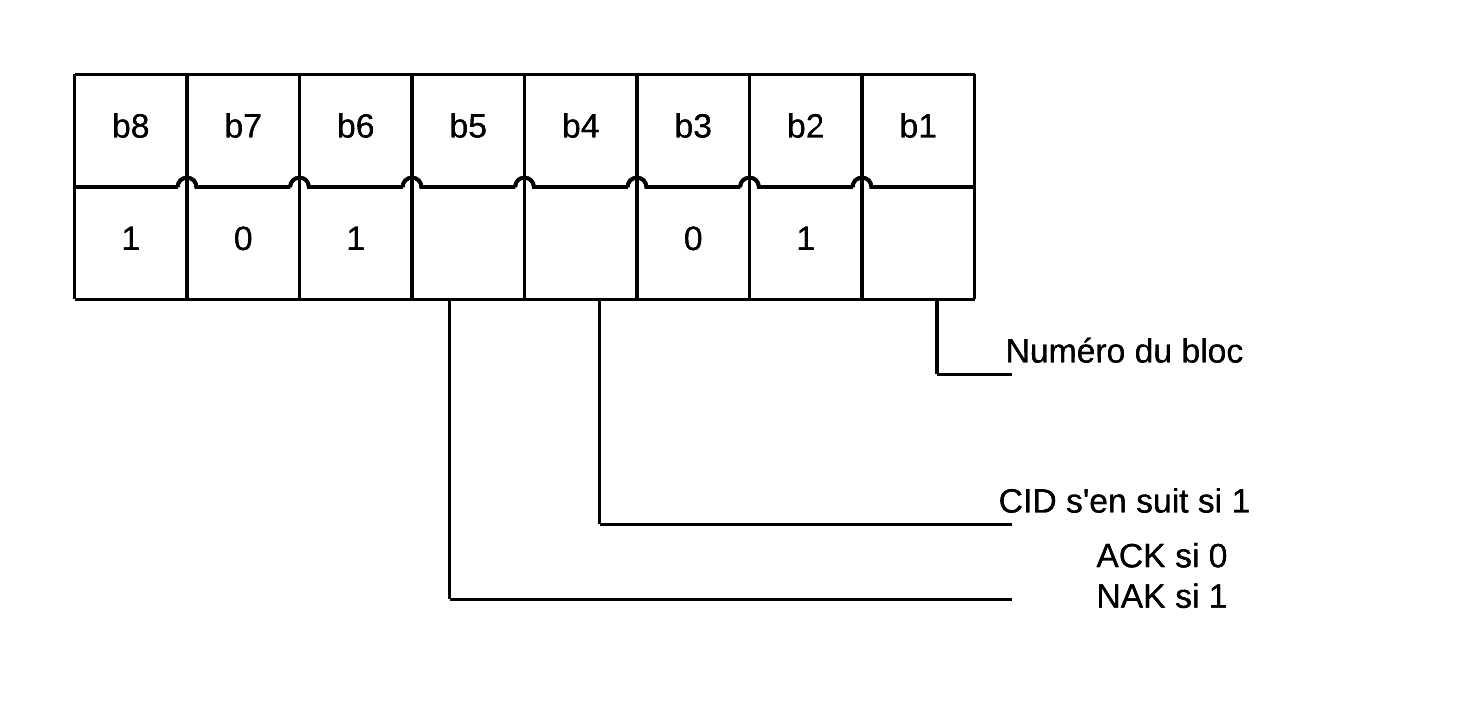
\includegraphics[scale=1]{images/rblock.png}
\caption{Structure binaire d'un R-Block}
\label{fig:R-Block}
\end{figure}

\begin{figure}[h!]
\centering
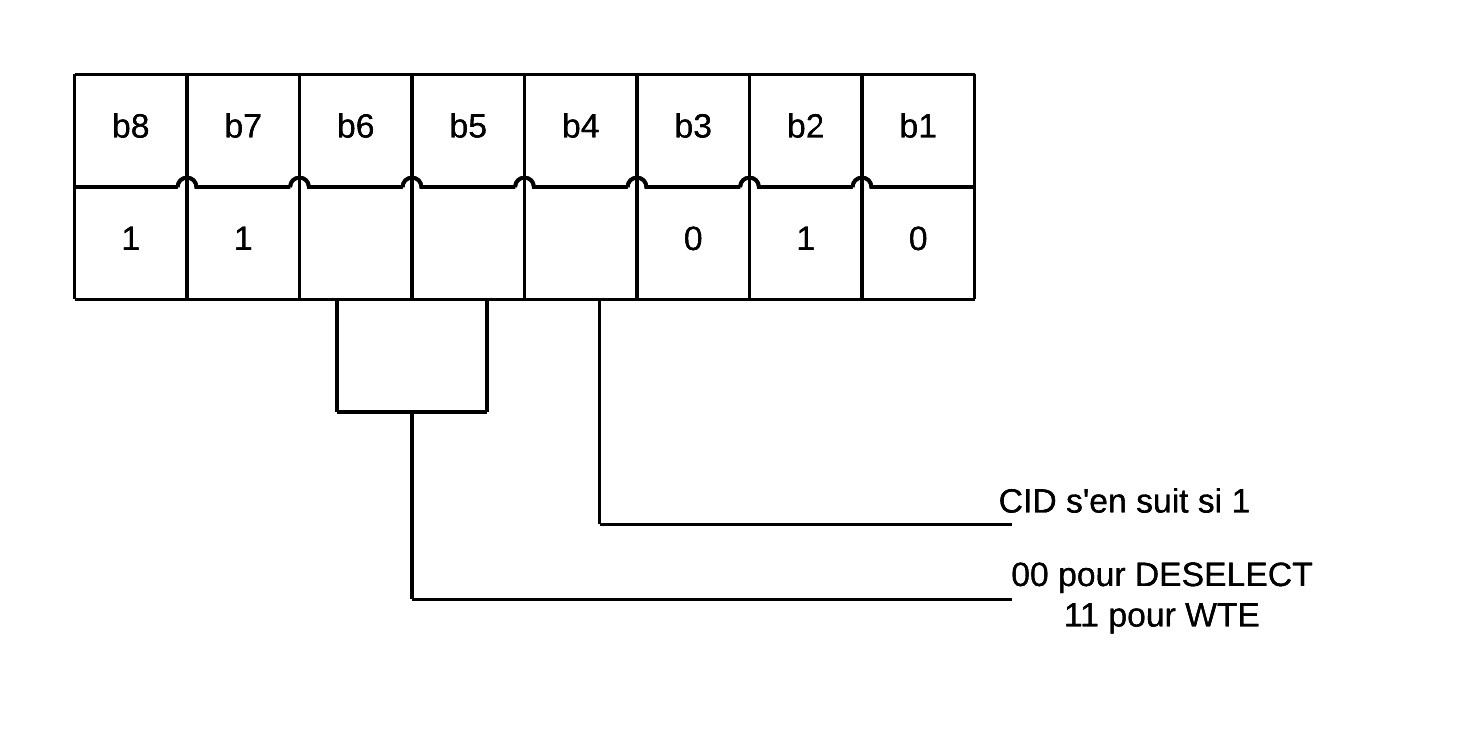
\includegraphics[scale=1]{images/sblock.png}
\caption{Structure binaire d'un S-Block}
\label{fig:S-Block}
\end{figure}
\paragraph{CID[optionnel]:}
CID (Card IDentifier) est un octet attribué par le PCD et qui sert à identifier un PICC. La manière dont le PICC gère un CID est décrite dans ce qui suit:

Un PICC qui ne supporte pas les CID\footnote{Comme l'AS3953} doit l'ignorer.

Un PICC qui supporte le CID doit:
\begin{itemize}
\item Répondre à un bloc contenant un CID en utilisant le même CID.
\item Ignorer les blocs contenant d'autres CID que celui utilisé à l'initiation de la communication.
\item Répondre avec un bloc sans CID s'il reçoit un CID nul.
\end{itemize}

\paragraph{NAD[optionnel]:}

Non supporté par l'AS3953\footnote{On laisse le lecteur curieux découvrir son utilité et son fonctionnement dans l'ISO-14443-3.}.

\subsubsection{Champ d'information [INF][optionnel]:}

Le champ INF est utilisé pour envoyer les informations de la couche applicatif du PICC au PCD et inversement. La longueur de ce champ est calculée  en fonction des octets qu'il contient.

\subsubsection{L'epilogue:}
Ce champ contient le CRC du bloc envoyé, son calcul est détaillé dans l'ISO/IEC 14443-3. Il est calculé automatiquement par la puce AS3953.

La structure de données du BTP qu'on vient de présenter a été programmée et intégrée dans G3OS durant ce stage. Dans ce qui suit on présente l'aspect dynamique du système NFC. On détermine un certain nombre de scénarios auxquels le système doit répondre. 

\subsection{Conception dynamique des couches logicielles et développement}
\textit{ Dans ce qui suit la notation $I(X)$ désigne un I-Block avec un numéro de bloc X. On utilise le diagramme de séquence UML pour modéliser les scénarios possibles. Tous les scénarios suivants ont été programmés et intégrés dans G3OS lors de ce stage}

Comme dans n'importe quel RTOS. La NFC correspond à une tâche indépendante. L'ordonnanceur de G3OS reçoit un signal d'interruption de la puce NFC, acquitte l'interruption et lance la tâche correspondante. Et c'est alors à la tâche de découvrir pourquoi elle a été lancée en lisant le registre principal des interruptions de la puce NFC. Toutes les communications entre le micro-contrôleur (MSP430) et la puce NFC (AS3953) s'effectue en SPI(interface série).

En plus des registres, l'AS3953 contient une EEPROM(Electrically Erasable Programmable Read-Only Memory) de 32 mots de 32 bits et une file FIFO (First In First Out) de 32 octets qui permet de stocker temporairement les informations à transmettre dans les deux sens. Tous ces éléments sont accessible en SPI\footnote{Voir Chapitre1 pour comprendre le fonctionnement}.

Lorsqu'on veut écrire un mot dans la FIFO par exemple, il faut fabriquer une suite de bits constituée de:
\begin{itemize}
\item Un octet pour indiquer le mode de communication. C'est le mot qui permet au microcontrôleur d'indiquer à la puce NFC ce qu'on veut faire. Tous les modes de communication sont disponible sur la datasheet de l'AS3953. Pour écrire un mot dans la FIFO par exemple, le mode correspondant est 1000 0000
\item L'adresse du mot de la FIFO qu'on veut écrire. La plage d'adresse de la FIFO est entre 0000 0000 et 0010 0000
\item Le mot qu'on veut écrire.
\end{itemize}
Donc la suite de bits: 1000 0000 0010 0000 1111 0000 envoyée en SPI correspond à une écriture du mot 1111 0000 dans le dernier mot de la FIFO(32ème mot).
\begin{figure}[h!]
\centering
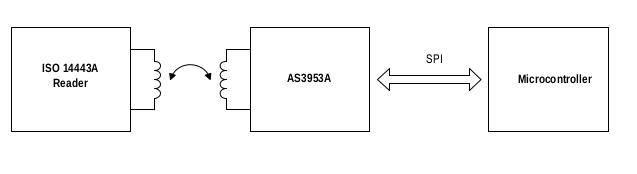
\includegraphics[scale=0.8]{images/blockdiagram.png}
\label{fig:blockdiagram}
\caption{Schéma en fonctionnement global de l'AS3953}
\end{figure}

Ainsi toutes les communications entre le micro-contrôleur et la puce NFC s'effectuent de la même façon: constituer un mot contenant un octet pour le mode de communication\footnote{Lire/Ecrire l'EEPROM, Lire/Ecrire les registres et Lire/Ecrire la FIFO}, suivi d'un mot pour indiquer l'adresse qu'on veut lire ou écrire et finalement le mot qu'on veut écrire pour l'écriture et rien pour la lecture.

L'AS3953 implémente aussi un certain nombre de commandes dites commandes directes. Les commandes directes permettent au micro-contrôleur de notifier la puce NFC

\begin{itemize}
\item Clear: arrêter toutes les activités et effacer tous les mots de la FIFO.
\item Transmit: Transmettre les données stockées dans la FIFO à l'autre dispositif (du PICC au PCD et inversement).
\item Go2halt: arrêter la communication avec le dispositif.
\item setDefault: retourner à l'état par défaut de la puce (état initial).
\end{itemize}

Les deux commandes qui nous intéressent le plus sont: Transmit et Go2halt. La première permet d'envoyer le contenu de la FIFO au dispositif NFC destinataire et la deuxième arrêter la communication avec celui ci.

Lorsqu'on reçoit un message d'un autre dispositif. Un signal d'interruption permet de notifier le micro-contrôleur qu'un dispositif à initier le processus de communication et a passé les trois premiers niveaux de l'ISO/IEC 14443 et qu'il veut initier un échange de message avec le micro-contrôleur. Dès que ce signal d'interruption est acquitté, l'ordonnanceur lance la tâche NFC, qui commence par lire le registre des interruptions pour s'assurer qu'il s'agit bien d'une initiation de communication et que le dispositif en question a passé les 3 premiers niveaux de la norme NFC sans problèmes. Dès lors, il peut lire le premier message reçu de la FIFO et répondre en écrivant un mot dans la FIFO et en exécutant la commande Transmit pour envoyer le message.

L'échange des messages entre deux dispositifs doit se faire en respectant le FWT (Frame Waiting Time) qui est le temps dans lequel un dispositif doit renvoyer un message en réponse à un bloc reçu. Si aucune réponse n'est initiée dans la période définit par le FWT, la connexion est arrêtée. La valeur par défaut du FWT et de 2000 ms.

\begin{figure}[h!]
\centering
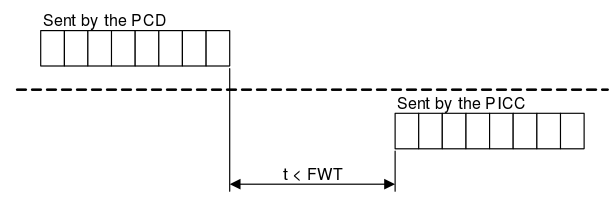
\includegraphics[scale=0.65]{images/fwt.png}
\caption{le Frame Waiting Time}
\end{figure}

Le 4ème niveau de l'ISO/IEC 14443 oblige les dispositifs NFC à utiliser le protocole de transmission des blocs pour échanger les messages. Dans ce qui suit quelques scénarios de communication. On fait abstraction sur la manière dont l'échange s'effectue (C'est ce qu'on a expliqué précédemment) et on se concentre sur la nature des blocs envoyés pour chaque scénario. Voir la conception statique des couches logicielles pour plus d'informations sur la structure des blocs.

\subsubsection{Vérification de la présence et la compatibilité du PICC}
Le PCD peut vérifier la présence d'un PICC et sa compatibilité avec la norme ISO-14443 en échangeant des I-Block ou des R-Block suivant le diagramme de séquence Figure\ref{fig:presencecheck}.

\begin{figure}[h!]
\centering
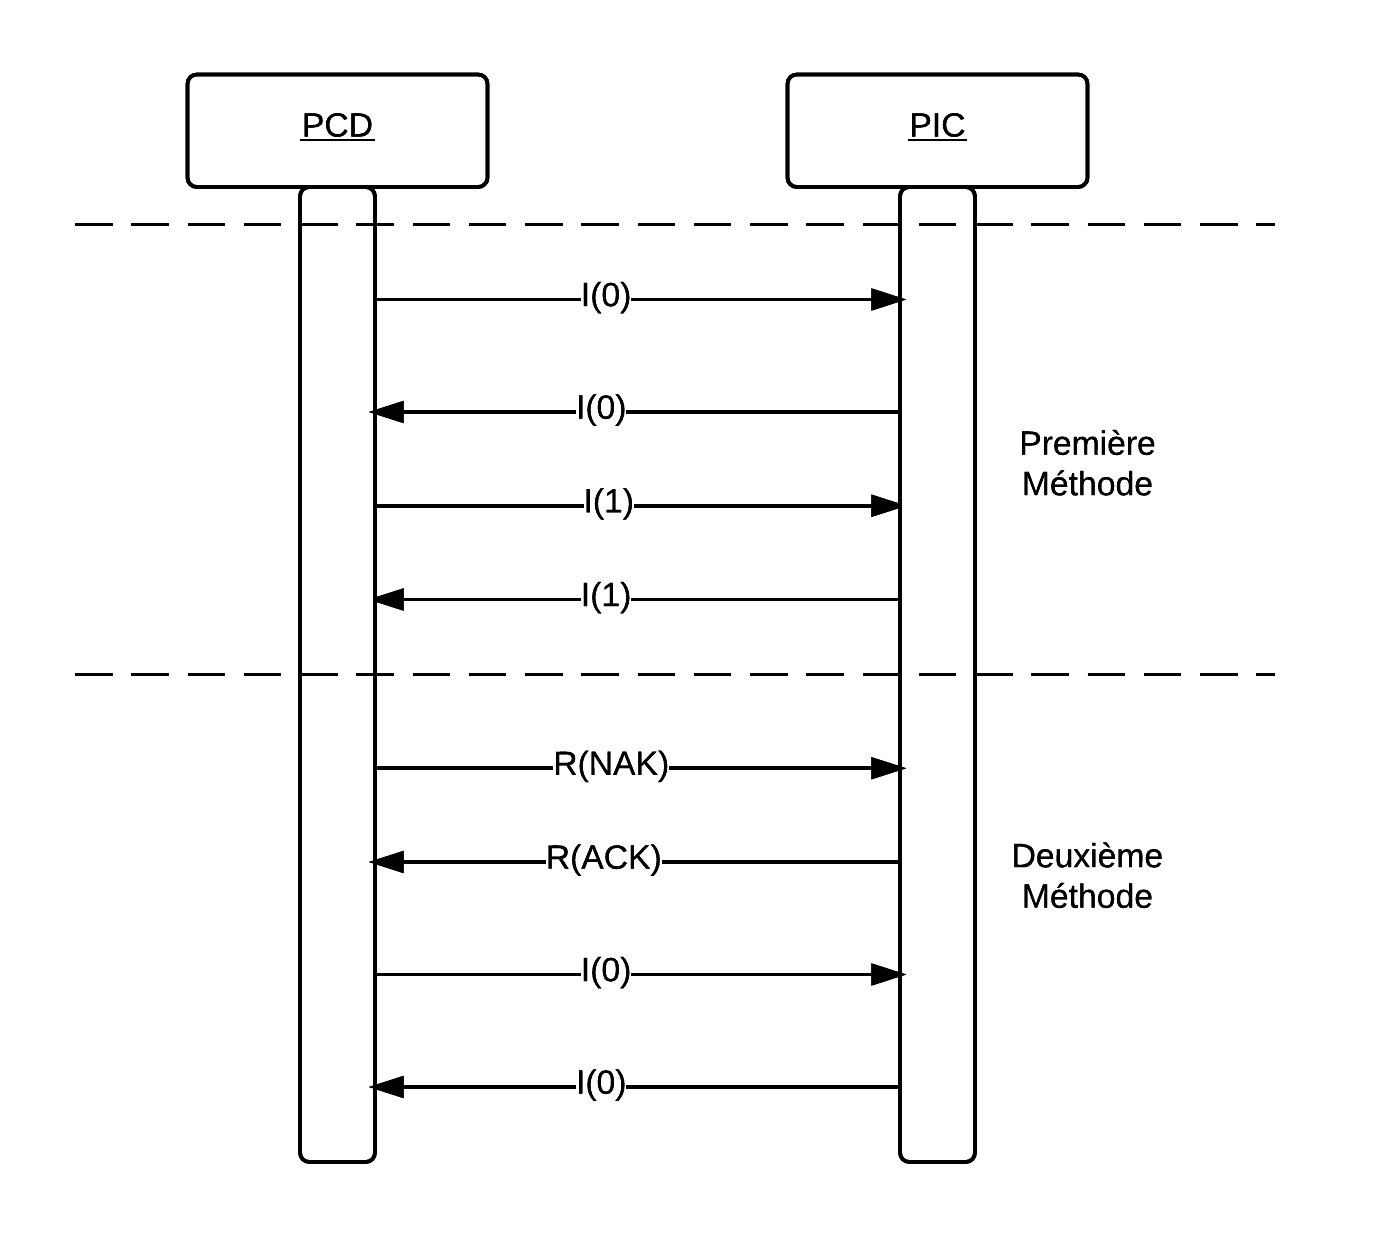
\includegraphics[scale=0.9]{images/presencecheck.png}
\label{fig:presencecheck}
\caption{Diagramme de séquence pour la vérification de la présence d'un PICC compatible ISO/IEC 14443}
\end{figure}

\subsubsection{DESELECT:}
DESELECT est la commande envoyée par le PCD pour informer le PICC de la fin de la transmission. Comme nous avons évoqué précedemment, cette commande est codé dans un S-Block. L'équivalent binaire du prologue d'une commande DESELECT est: 1100 0010. Sachant que le 4ème bit peut être 1 si le CID s'en suit. La Figure\ref{fig:deselect} présente le diagramme de séquence correspondant.

\begin{figure}[h!]
\centering
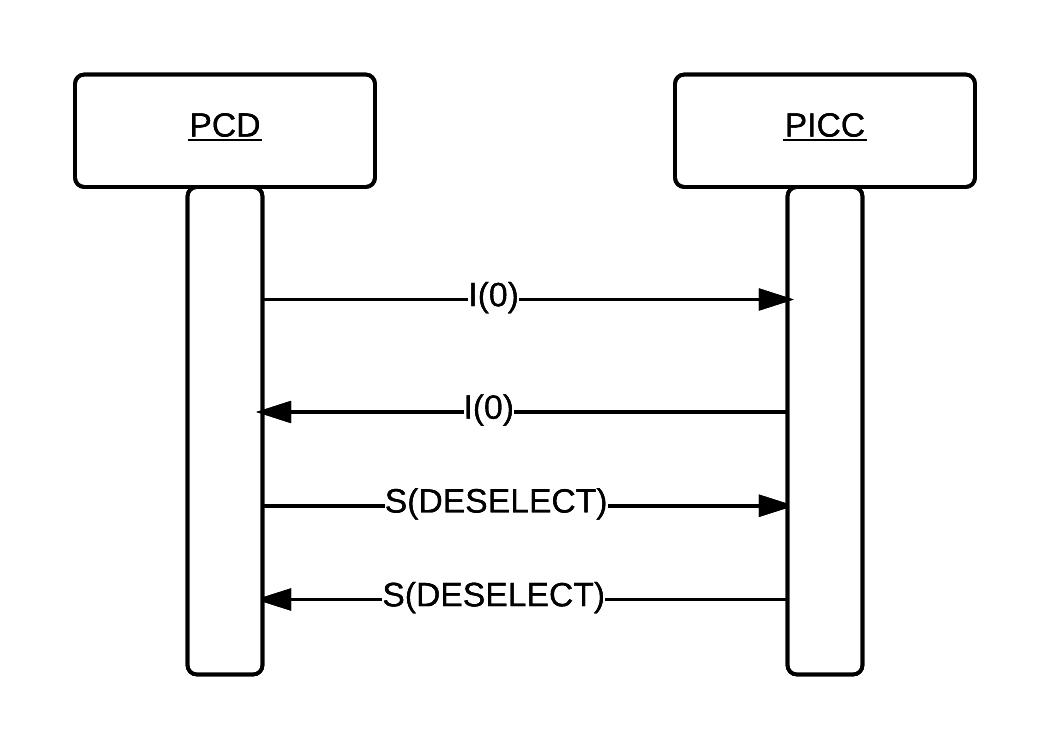
\includegraphics[scale=0.9]{images/deselect.png}
\label{fig:deselect}
\caption{Diagramme de séquence pour l'échange d'une commande DESELECT}
\end{figure}

\subsubsection{Échange de données:}
Pour échanger des données entre les PCD et le PICC il faut utiliser des blocs de chaînage. Le chaînage est le mécanisme qui permet d'envoyer des données de la couche applicative. Il est activé en mettant le 5ème bit (b5) d'un I-Block à 1. Chaque bloc alors contient un champ d'informations INF. Chaque I-Block de chaînage contenant un champ d'information est alors notifié par le dispositif destinataire par un R(ACK).

\begin{figure}[h!]
\centering
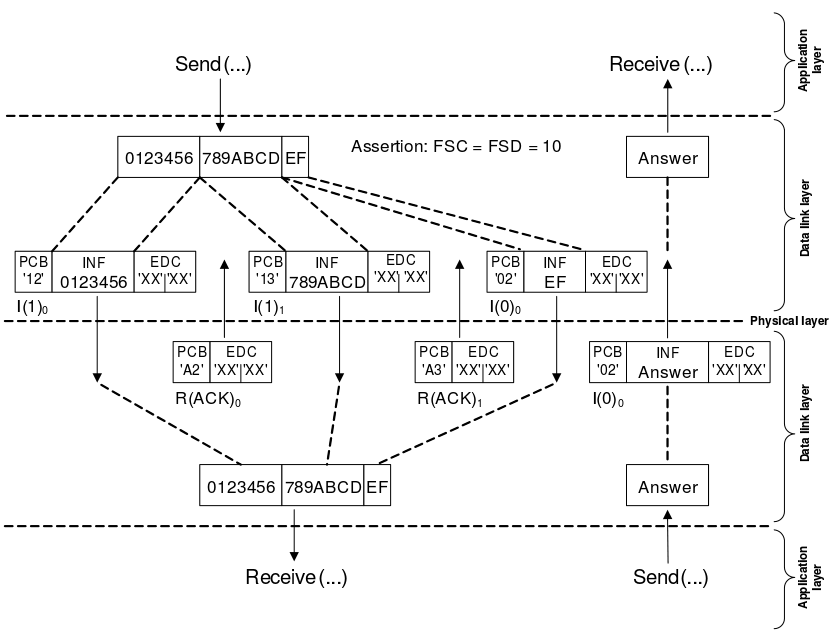
\includegraphics[scale=0.5]{images/chaining.png}
\label{fig:chaining}
\caption{Échange de blocs d'informations en utilisant le chaînage. crédit du schéma: OpenPCD.org}
\end{figure}

\subsubsection{Gestion des erreurs}
Lorsqu'une erreur survient lors de la transmission des blocs, l'état du registre des erreurs est changé, 

%------------------------------------------------------------------------------------
%------------------------------------------------------------------------------------
\evenchapter[Conception, développement et déploiement d'un système de mise à jour automatique destinée au système Géocube:]{Conception, développement et déploiement d'un système de mise à jour automatique destinée au système Géocube:}
\textit{ Dans ce chapitre plusieurs diagrammes UML(Unified Modelling Language) sont utilisés pour simplifier la conception du système de mise à jour au lecteur. Pour plus d'informations sur le langage voir []. Le système de mise à jour développé fut baptisé Sharokey}
\section{Étude du besoin:}
Le besoin se fait ressentir de plus en plus au sein de la société Kylia de disposer d'un système permettant aux clients qui ont acheté un système Géocube  d'effectuer des mises à jour automatiques et de profiter ainsi des améliorations éventuelles qui seront amenées aux couches logicielles des produit sans pour autant procéder à un rappel de celui ci.

En plus de la gestion des mises à jour, ce système doit être au coeur de plusieurs métiers, permettant de coordonner le travail entre le développeur, l'administrateur système, l'opérateur commercial et les clients désirant profiter des dernières améliorations portées sur les couches logicielles.

\begin{figure}[h!]
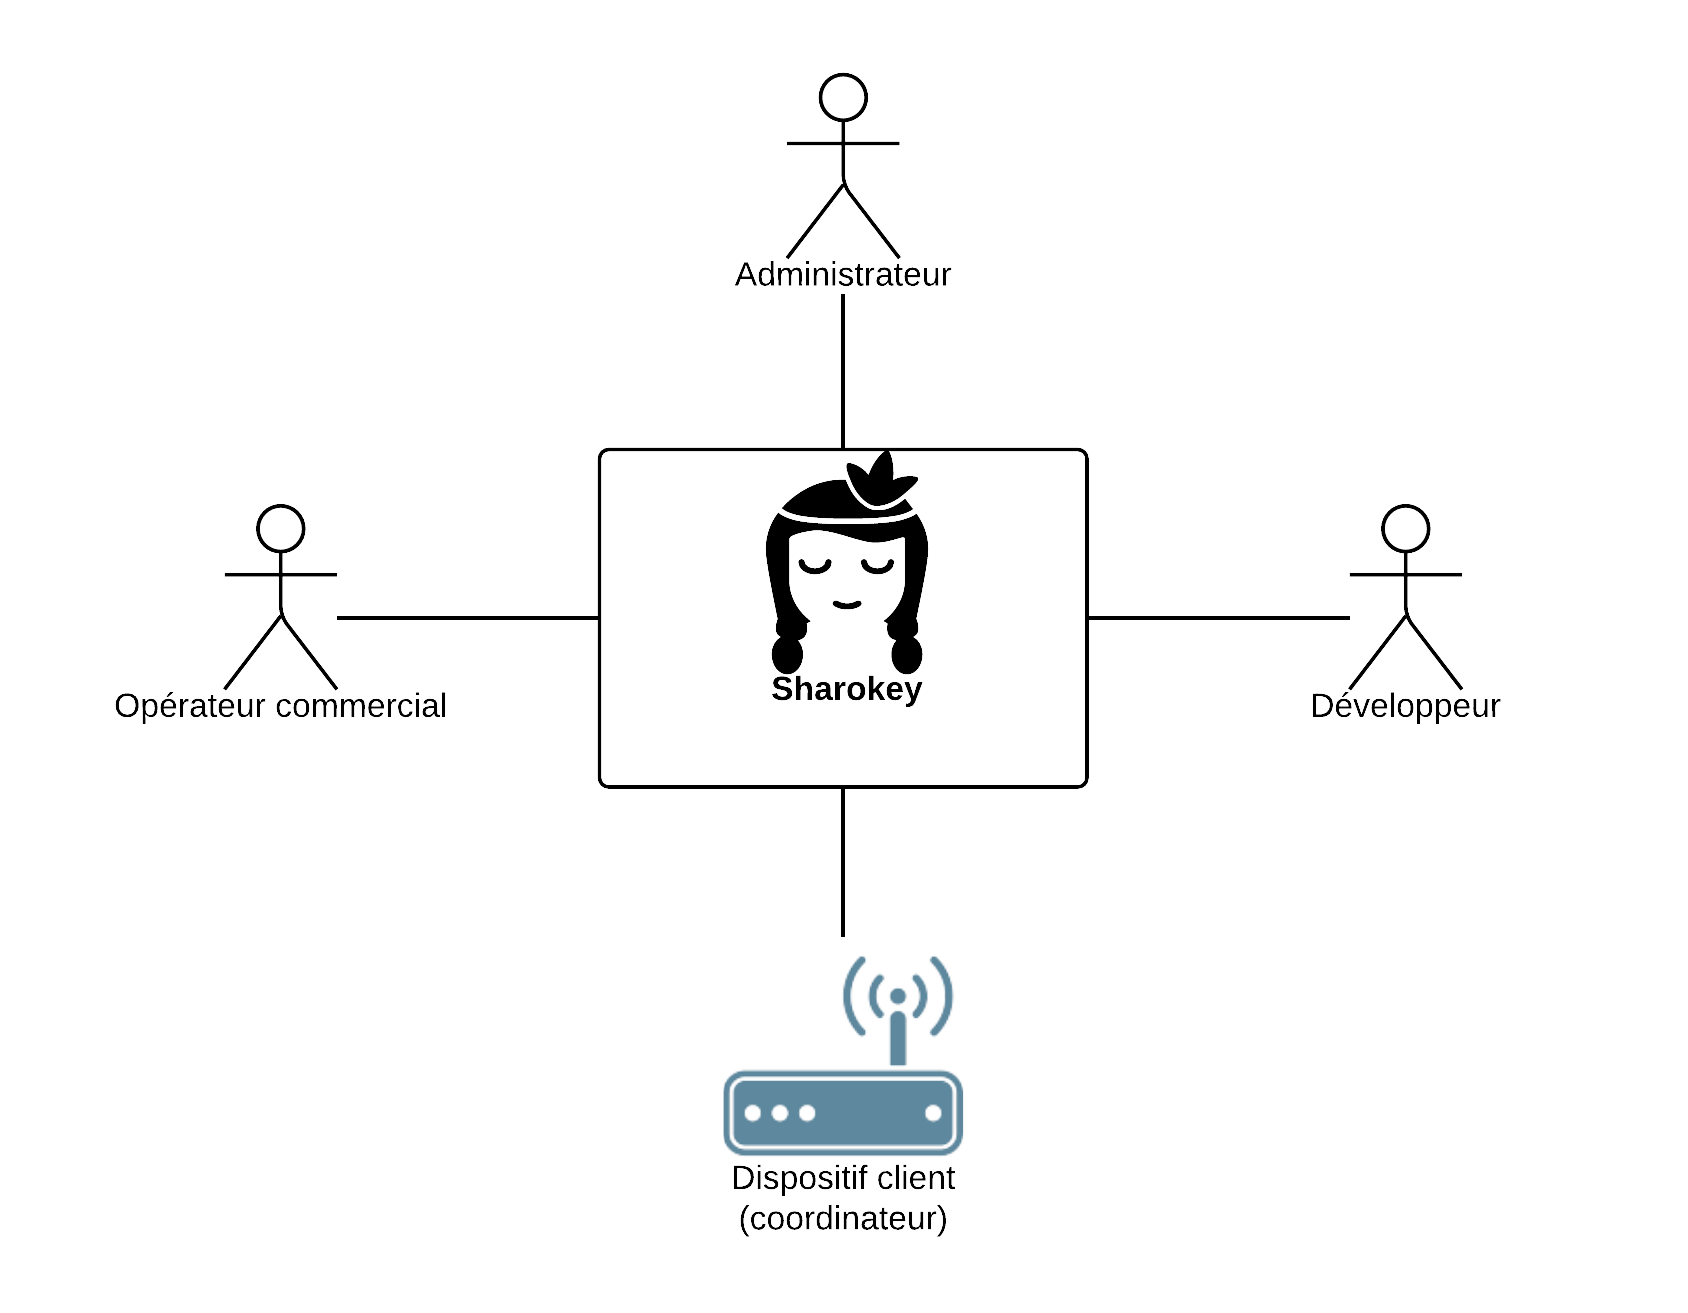
\includegraphics[scale=0.9]{images/context_general.png}
\label{fig:context_statique}
\centering
\caption{Diagramme de contexte statique}
\end{figure}

De la Figure\ref{fig:context_statique} on définit les acteurs suivants:
\begin{itemize}
\item Opérateur commercial: Personne qui procède à la vente des systèmes Géocubes et des licences de mise à jour. Une licence a un date de début et une date de fin. Elle détermine la période ((pour laquelle)) le client à le droit de profiter du support logiciel à travers la mise à jour de son dispositif.
\item Développeur: Personne responsable de l'alimentation continue du système en versions.
\item Administrateur: Personne responsable de l'administration et la supervision du système de mise à jour.
\item Coordinateur: Dispositif client destiné à être mis à jour.
\end{itemize}

Ce système doit en plus présenter les particularités suivantes:
\begin{itemize}
\item La supervision et l'administration du système doit être simplifiée à travers des interfaces homme-machine.
\item 
\item Les logs du système doivent être expressifs et facilement accessible par l'administrateur.
\item Les requêtes du client et les réponses du serveur doivent être sécurisées.
\end{itemize}

\section{Conception statique}
La Figure\ref{fig:use_case} résume les cas d'utilisation de Sharokey.

\begin{figure}[h!]
\centering
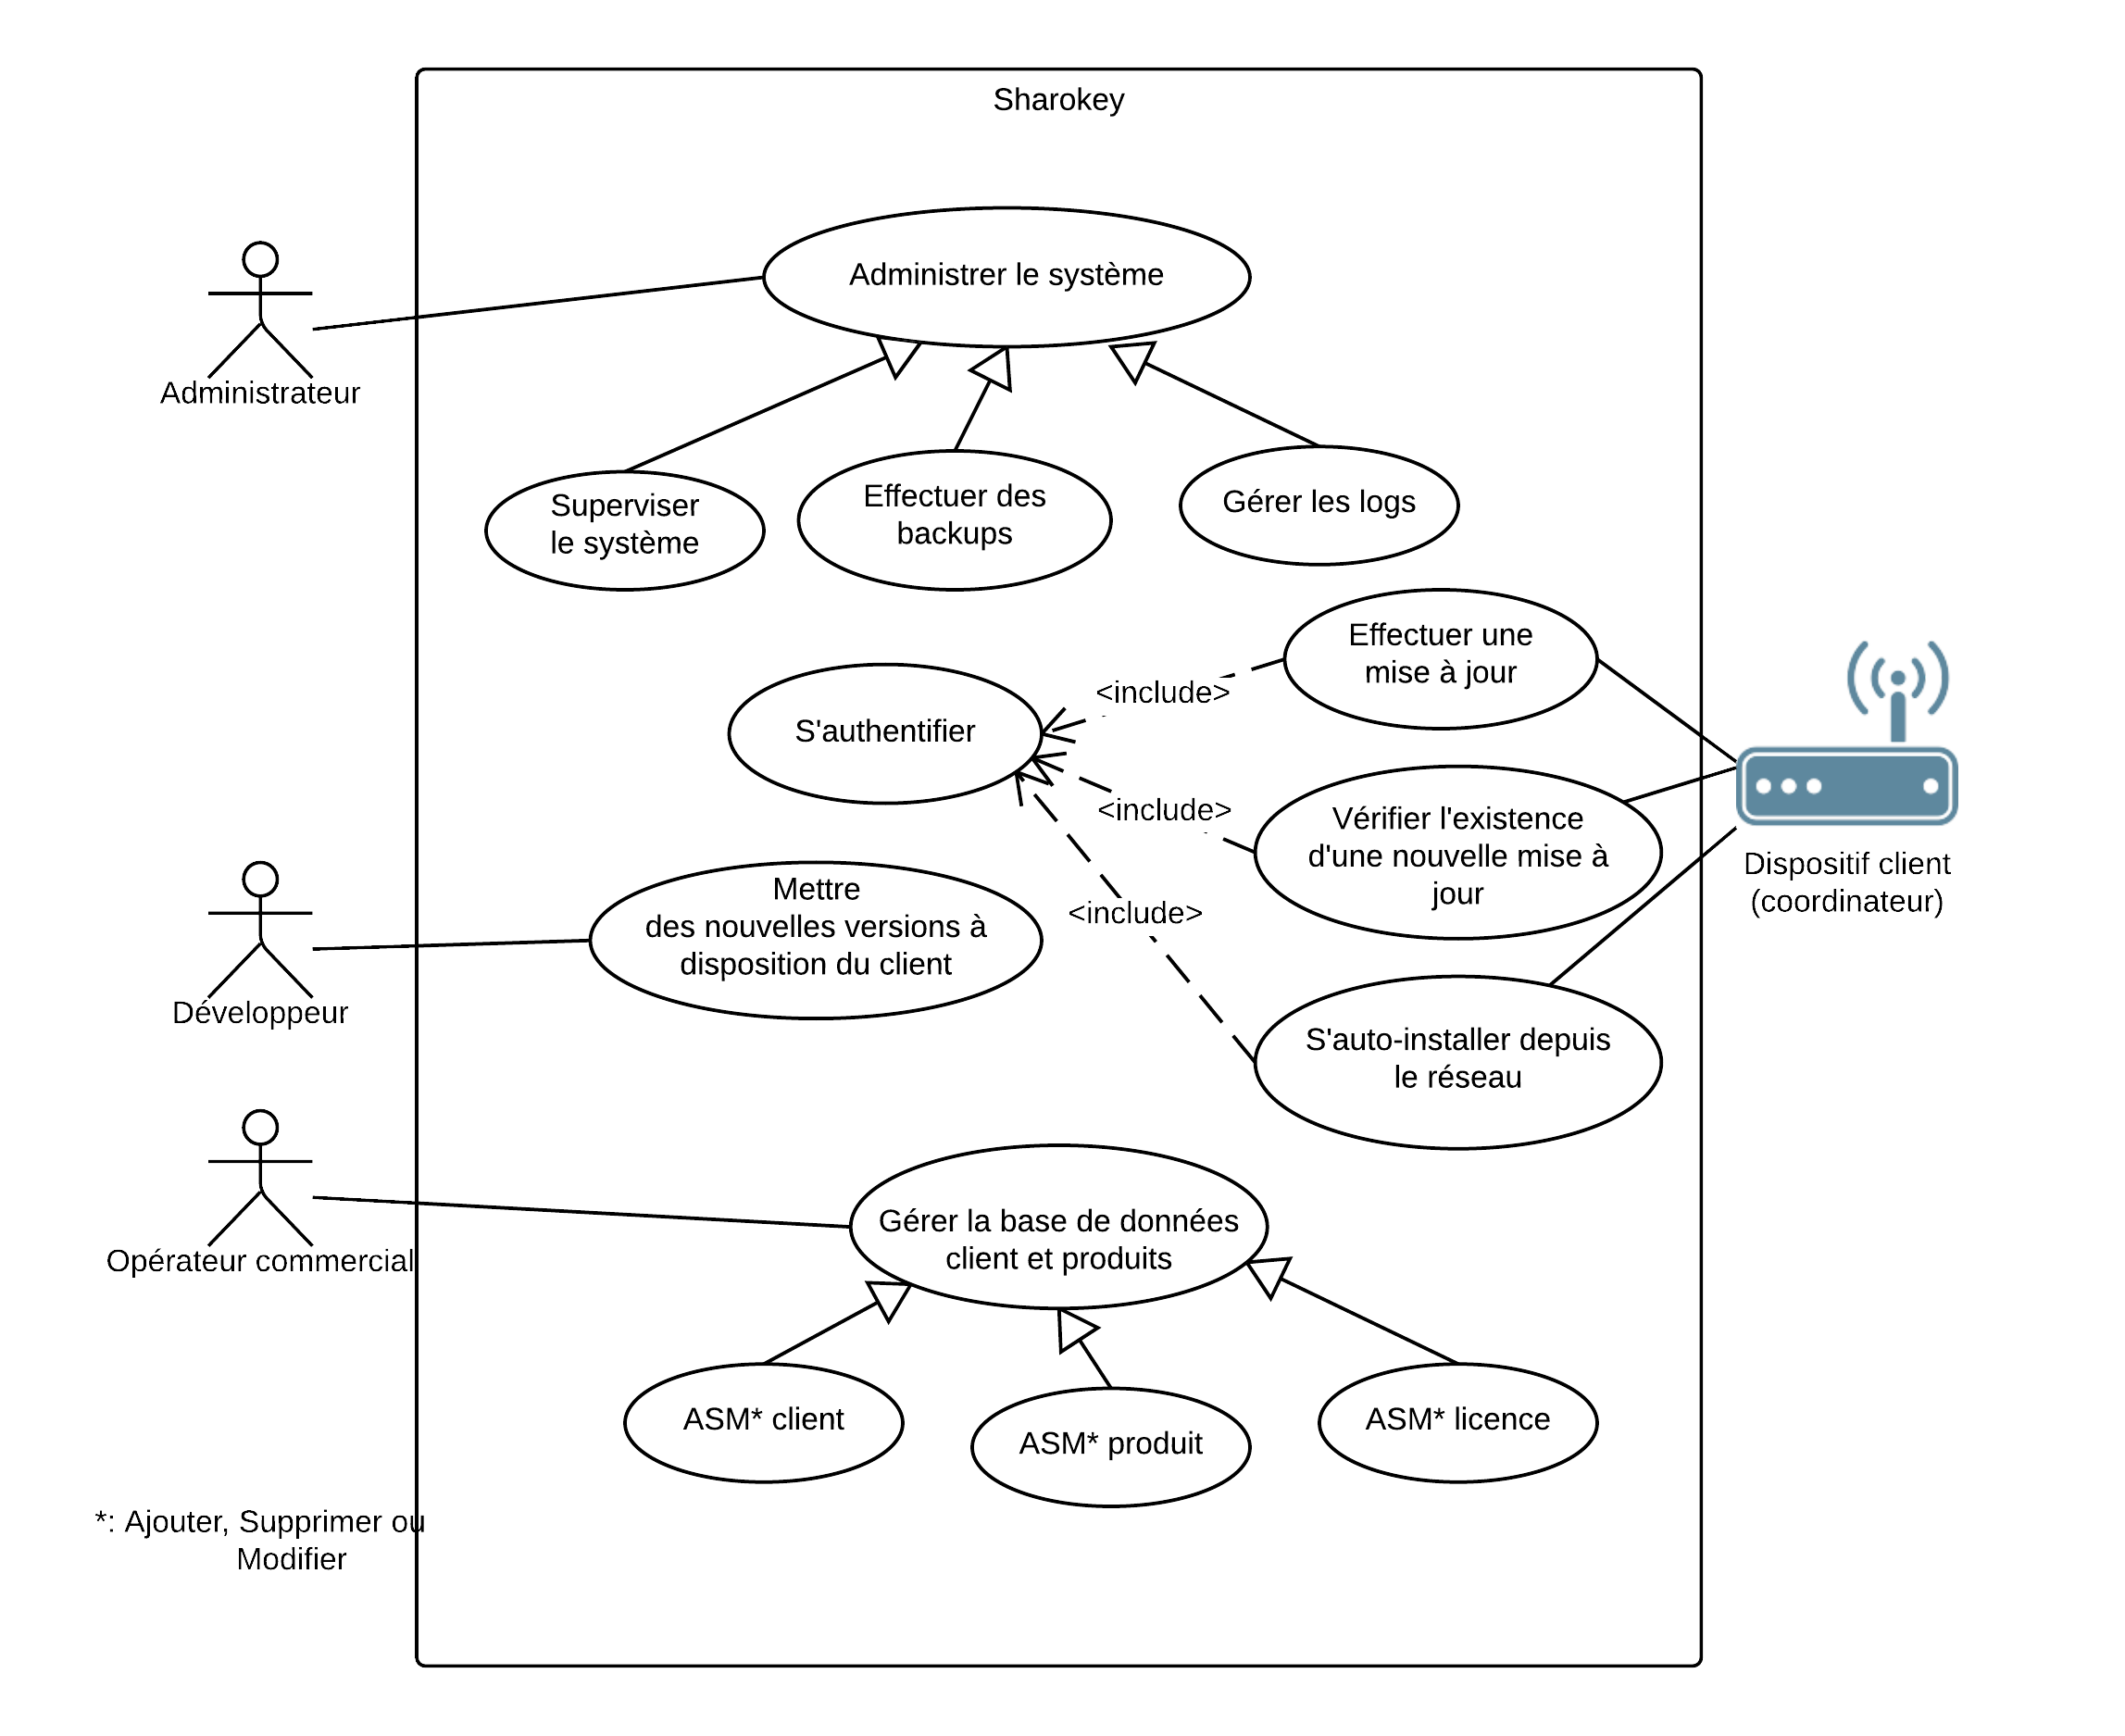
\includegraphics[scale=1]{images/use_case_sharokey.png}
\label{fig:use_case}
\caption{Diagramme UML des cas d'utilisation de Sharokey}
\end{figure}

La modélisation de la base de donnée est présentée dans la Figure\ref{fig:mpd}. On définit alors les entités suivantes:
\begin{itemize}
\item client: Personne physique qui effectue la commande d'un produit, elle est identifiée par IDC (clef primaire ID Client). Cette personne peut appartenir à une institution (entreprise ou organisme étatique), Les autres champs de la table servent à identifier les informations nécessaires au contact: Nom, Prénom, Téléphone, E-mail et un commentaire qui est laissé au soins de l'opérateur commercial.
\item product: C'est le coordinateur qui est destiné à recevoir les mises à jour. Il est identifié par son Part-Number (IDP). On lui attribue en plus un nom qui est généralement celui de la marque du fabriquant.
\item license: Entité qui établie la relation entre la table product et la table client, en utilisant des clés étrangères vers leurs identifiants. Elle attribue à chaque client une licence de mises à jour sur un produit pour une durée comprise entre une date de début (start date) et une date de fin (end date).
\item software: C'est la table qui contient toutes les mises avec les numéros de versions correspondants. Elle contient une clef étrangère vers la table product, puisque chaque mise à jour est destinée à un produit particulier. chaque mise à jour est identifiée par une version majeure, une version mineure et une version de patchs. La version 1.0.5 correspond alors à la version majeure 1, la version mineure 0 et la version de patchs 5. En plus, chaque mise à jour a un type qui peut être soit V (pour version), ou P pour (patch). La différence réside dans la pertinence des améliorations portées.
\item Les triggers: Deux triggers pour écouter les événements des tables: client et product.
\end{itemize}

\begin{figure}
\centering
\label{fig:mpd}
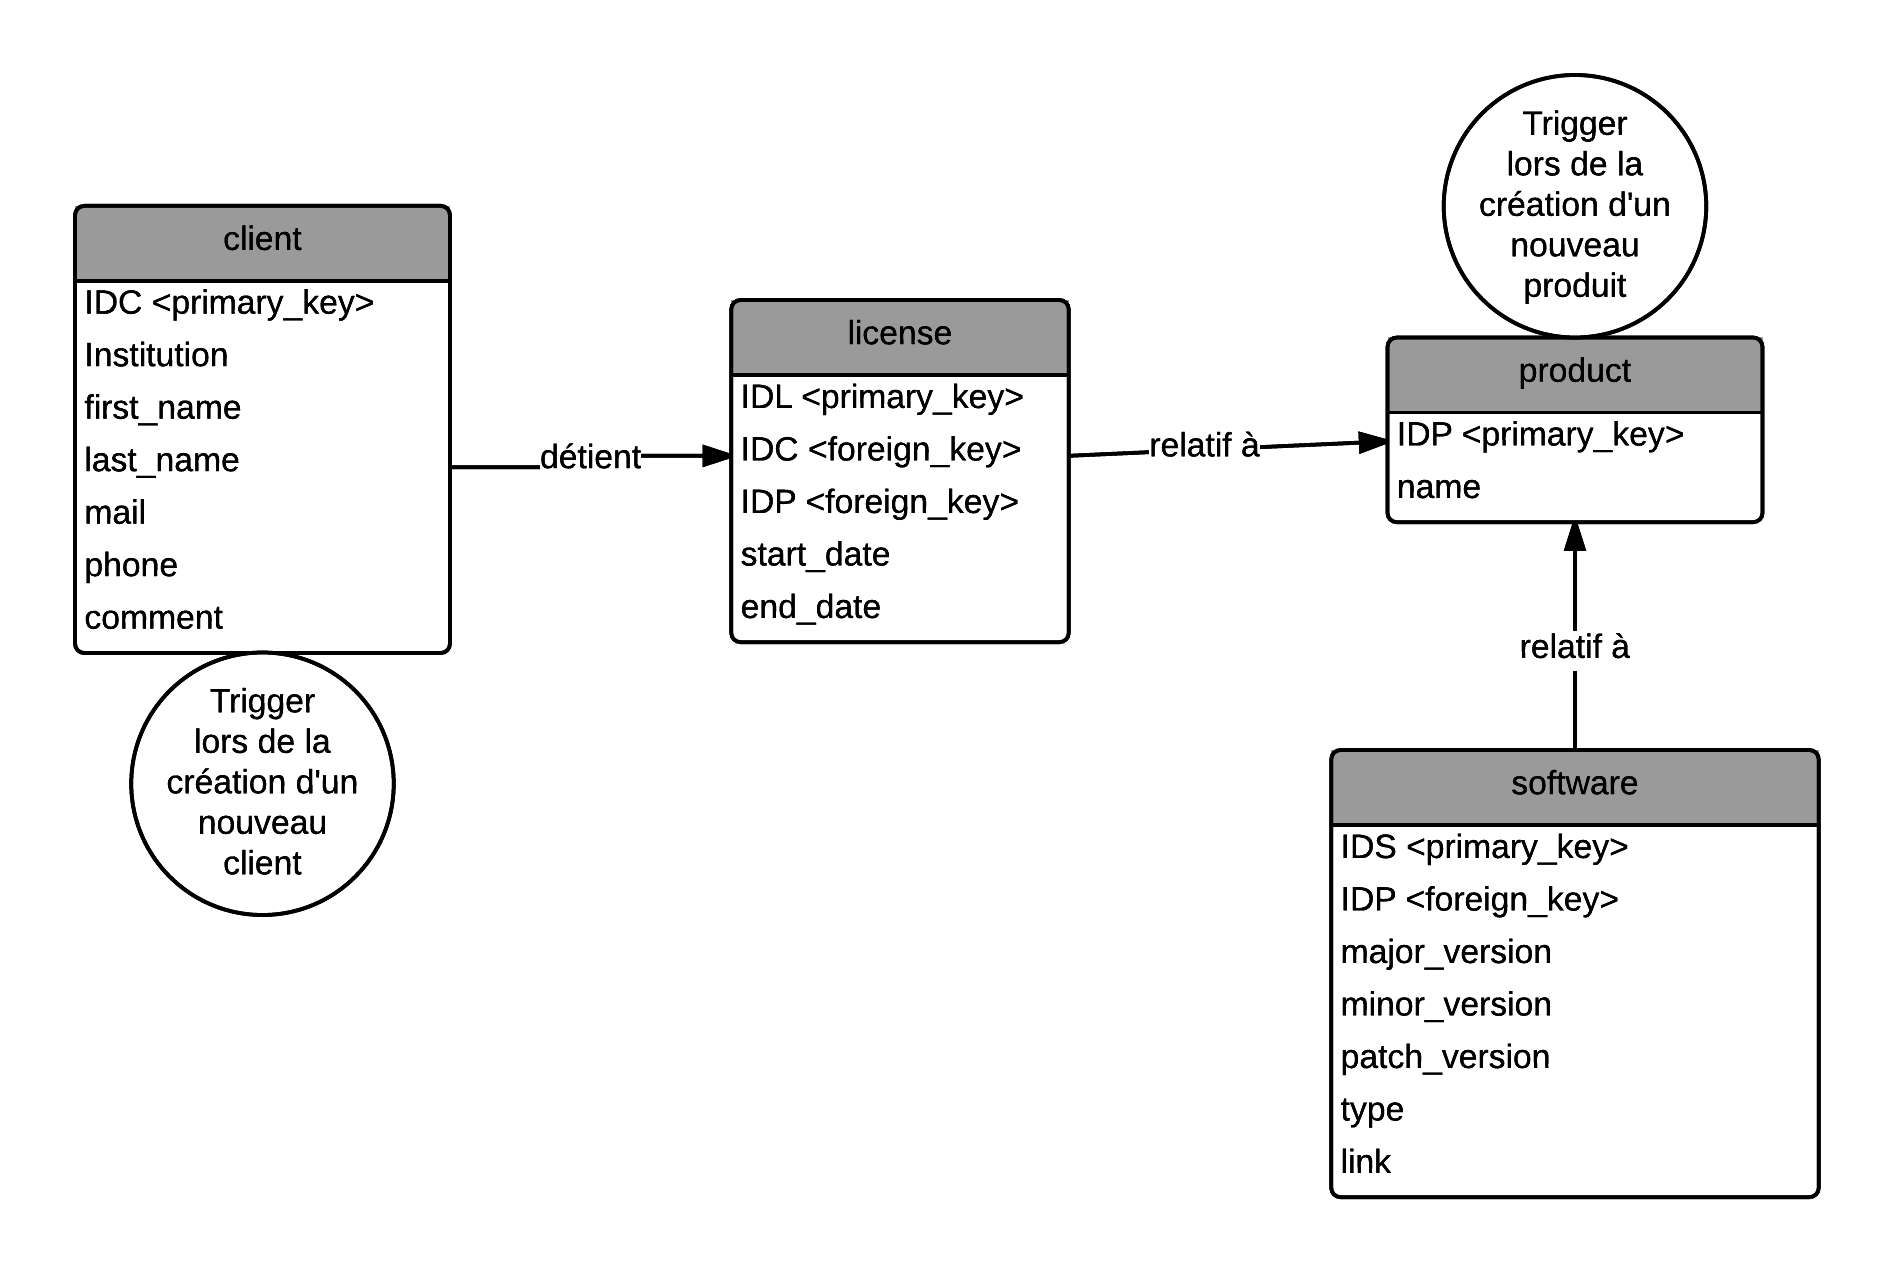
\includegraphics[scale=0.85]{images/MPD_sharokey.png}
\caption{MDP (Modèle Physique des Données) de la base de données Sharokey}
\end{figure}
\subsection{Format des mises à jour}

Une mise à jour est un script auto-extractible fabriqué en utilisant le programme Makeself. Un format de paquets a été conçu pour simplifier et automatiser la création des scripts de mise à jour. Ce format a un point d'entrée qu'on nomme "go.sh" et un répertoire de scripts et de données baptisé "installerScripts". go.sh est un script shell qui execute les scripts contenus dans installerScripts. la fabrication d'un éxecutable auto-extractible à partir de ces éléments en utilisant Makeself permet d'ajouter un mécanisme de vérification de l'intégrité du paquet de mise à jour avec une somme MD5.

\subsection{Architecture logicielle}
Sharokey est une solution informatique légère de mise à jour automatique pour les solutions informatiques propriétaires basés sur un système d'exploitation GNU/Linux et nécessitant une licence ou une autorisation pour faire les mises à jour. Il est basé sur une architecture client-serveur. Le client est codé entièrement en Shell pour garantir une portabilité sur toutes les distributions GNU/Linux et sur une grande panoplie d'architectures matérielles: Intel, ARM, MIPS, ... Le serveur est écrit en NodeJS. Ce choix garantie se portabilité sur les serveurs utilisant des OS type Windows ou GNU/Linux. Toute fois, il est fortement conseillé d'utiliser GNU/Linux. Les tests effectués jusqu'à ce jour n'ont porté que sur ce type d'OS.

\subsubsection{Client:}
Comme schématisé dans la Figure, La partie client est contituée d'un ensemble de paquets Kylia dont nous présentons les fonctionnalités ci-dessous:
\begin{itemize}
\item checker.kyl: Ce paquet renvoie trois codes possibles 0, 1 ou 2. 0 si le dispositif client arrive à se connecter au serveur mais aucune nouvelle mise à jour n'est disponible. 1 si le dispositif client arrive à se connecter au serveur et il y a une nouvelle mise à jour a effectué. 2 si le dispositif client n'arrive pas à se connecter à internet\footnote{Le code retour 2 est important pour le coordinateur des Géocubes, puisque ce dernier est dépendant d'internet. Ce code retour permet d'informer le client d'un souci de réseau}.
\item update.kyl: Ce paquet télécharge et éxécute les mises à jour, il change ensuite le numéro de la version courante dans le dispositif client pour l'adapter à celle du serveur.
\item zeus.kyl: Ce script a pour but d'automatiser la procédure d'installation d'un coordinateur "à la sortie d'usine".
\item phenix.kyl: Le but de ce paquet est de désintaller le coordinateur et de le réinstaller automatiquement, de partir d'une version minimaliste si une erreur survient.
\end{itemize}
\section{conception dynamique et développement}

\subsection{Sécurité du système}
La stratégie de sécurité instaurée pour Sharokey doit respecter les trois points suivants:
\begin{itemize}
\item S'assurer de l'identité du dispositif qui effectue la mise à jour
\item Les requêtes des clients et les réponses du serveur doivent être cryptés pour assurer la protection des paquets binaires lors de leur transition via le réseau.
\item S'assurer de l'intégrité des paquets envoyés par le serveur.
\end{itemize}
Dans cette perspective un système d'authentification par vérification de signature numérique sur la clef publique du client a été implémenté dans Sharokey. Une autorité de certification (KyliaCA) a été créée\footnote{Système cryptographique asymétrique en utilisant le standard RSA}. Son but est de signer la clef publique des clients pour garantir que leur dispositif a bien été vendu par Kylia. La génération des clés (privé et publique) des clients s'effectue d'une manière automatique dans Sharokey dès la création d'un nouveau client dans la base de données, d'ou le trigger Pl/PGSQL sur la table client(Figure\ref{fig:mpd}).

Pour créer une pair de clés (privé et publique signée) pour un client. Sharokey effectue trois opérations en utilisant les fonctions de la librairie OpenSSL:
\begin{itemize}
\item Créer une pair de clés aléatoires en utilisant le standard RSA et avec une longueur de 2048 octets\footnote{À ce jour, aucune faille n'est connue dans RSA pour les clés de longueur 2048 octets}
\item À partir de la clef publique, créer un CSR (Certificate Signature Request).
\item Signer le fichier CSR avec KyliaCA et générer ainsi une clef publique signée par l'autorité de certification de l'entreprise\footnote{Une autorité de certification est aussi une pair de clés publique-privé sauf qu'elle n'a été signée par aucune autre CA. Elle est auto-signée par elle même}.
\end{itemize}
Un tel mécanisme d'authentification assure que le dispositif qui veut effectuer la mise à jour provient de la société Kylia, et répond donc au premier point de sécurité précédemment énoncé.

Concernant le deuxième point relatif au cryptage des requêtes clients et des réponses du serveur. Sharokey oblige toutes les requêtes à passer par le protocole HTTPS pour garantir le cryptage des informations échangés entre le client et le serveur, et ceci en utilisant une cryptographie asymétrique basée sur l'échange mutuel des clés publiques.

Enfin, le troisième point relatif à l'intégrité des données transitant par le réseau est garantit par un mécanisme de checksum-MD5 implémenté par défaut dans le générateur de scripts auto-extractibles Makeself que Sharokey utilsie pour créer les paquets de mise à jour.

\subsection{Composants et interaction:}

\begin{figure}[h!]
\centering
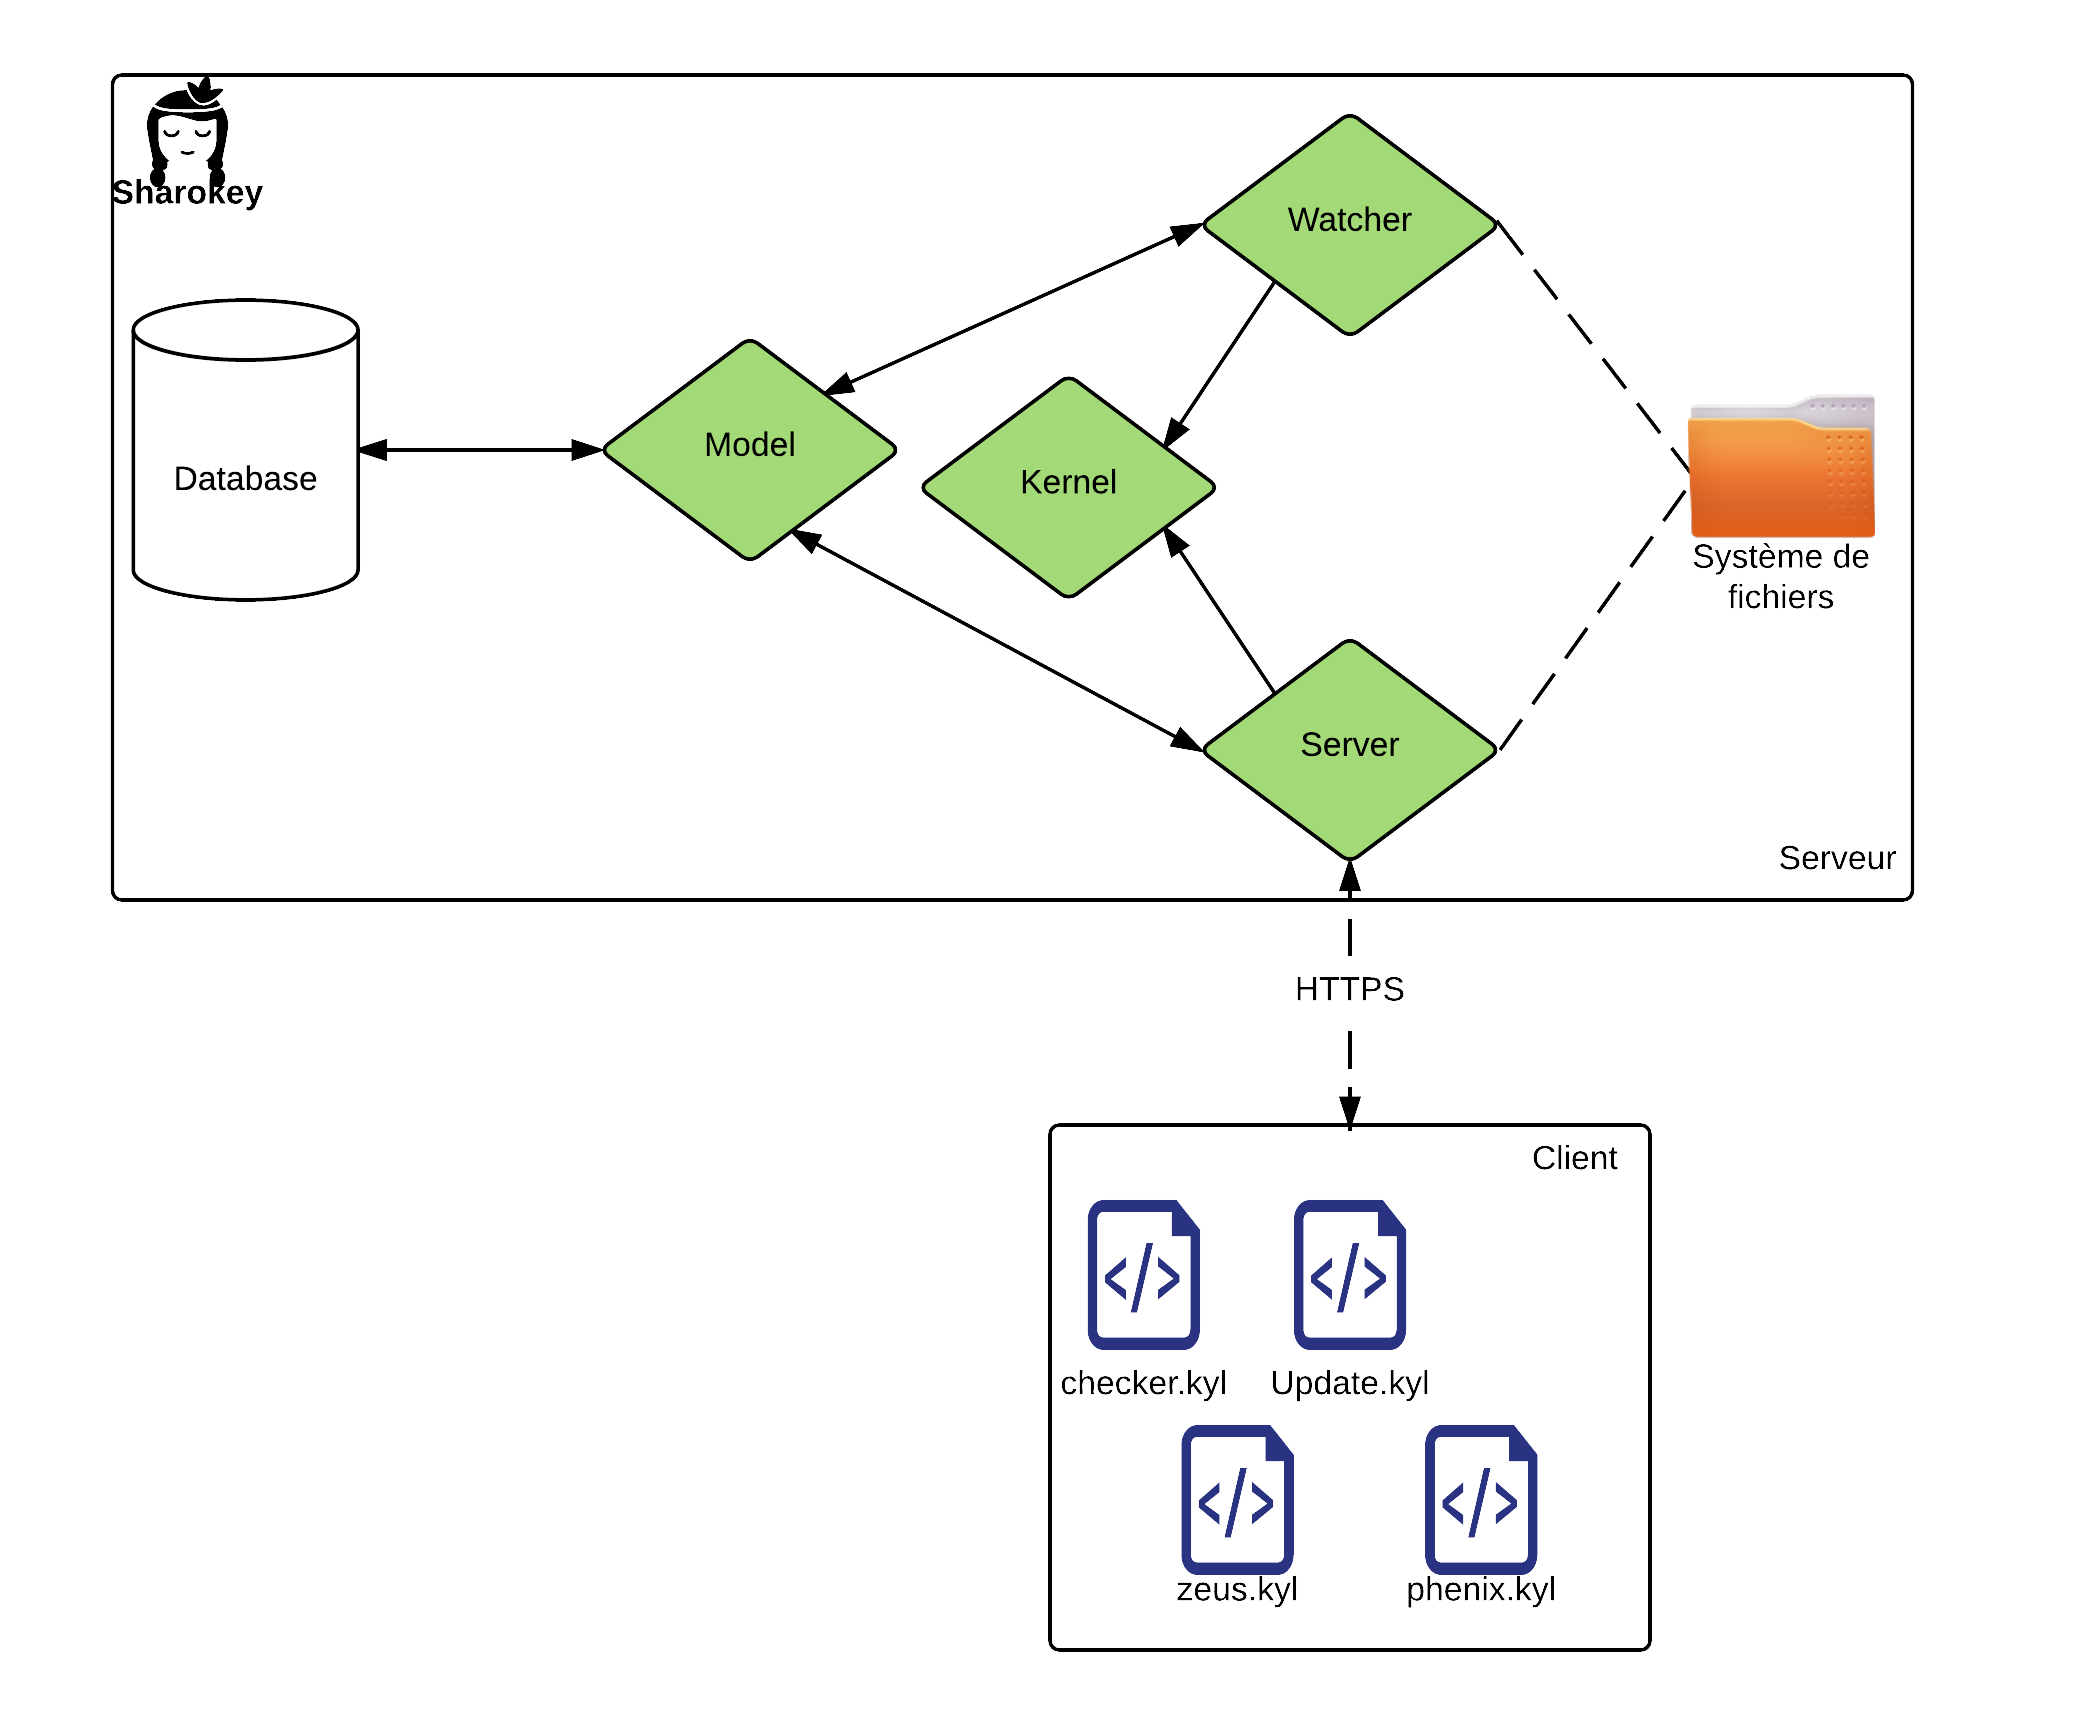
\includegraphics[scale=0.8]{images/composants.png}
\label{fig:composants}
\caption{Schéma des composants de Sharokey}
\end{figure}

La Figure\ref{fig:composants} présente les composants de sharokey. Dans ce qui suit le rlôe de chaque composant et son interaction avec les autres:

\begin{itemize}
\item Model: module NodeJS qui encapsule toute la logique liée aux opérations que les autres composants peuvent effectuer sur la base de donnée. Ainsi, si un module veut effectuer une opération sur la base de données, il devra passer par ce module.
\item Kernel: C'est le noyau NodeJS de Sharokey (l'API centrale) qui contient toutes les fonctions communes aux autres modules.
\item Watcher: C'est le composant le plus dynamique du système il écoute les triggers de la base de données effectue les modifications nécessaires sur le systèmes de fichier et vice-versa. Il encapsule aussi la logique liée à la sécurité et la génération automatique et signature des clés publiques et privés des nouveaux clients.
\item server: C'est le serveur NodeJS qui reçoit les requêtes des clients en HTTPS, vérifie la signature sur leurs clés publiques, vérifie leur droit d'effectuer des mises à jour, prépare et envoie la mise à jour sous format de scripts auto-extractible.
\end{itemize}

Le système a été conçu d'une manière modulaire, chaque composant peut vivre sur une machine à part l’interaction entre les modules s'effectue en utilisant TCP/IP.

Les Figures .... présentent les interactions entre les composants à travers des diagrammes de séquence UML.

\begin{figure}
\centering
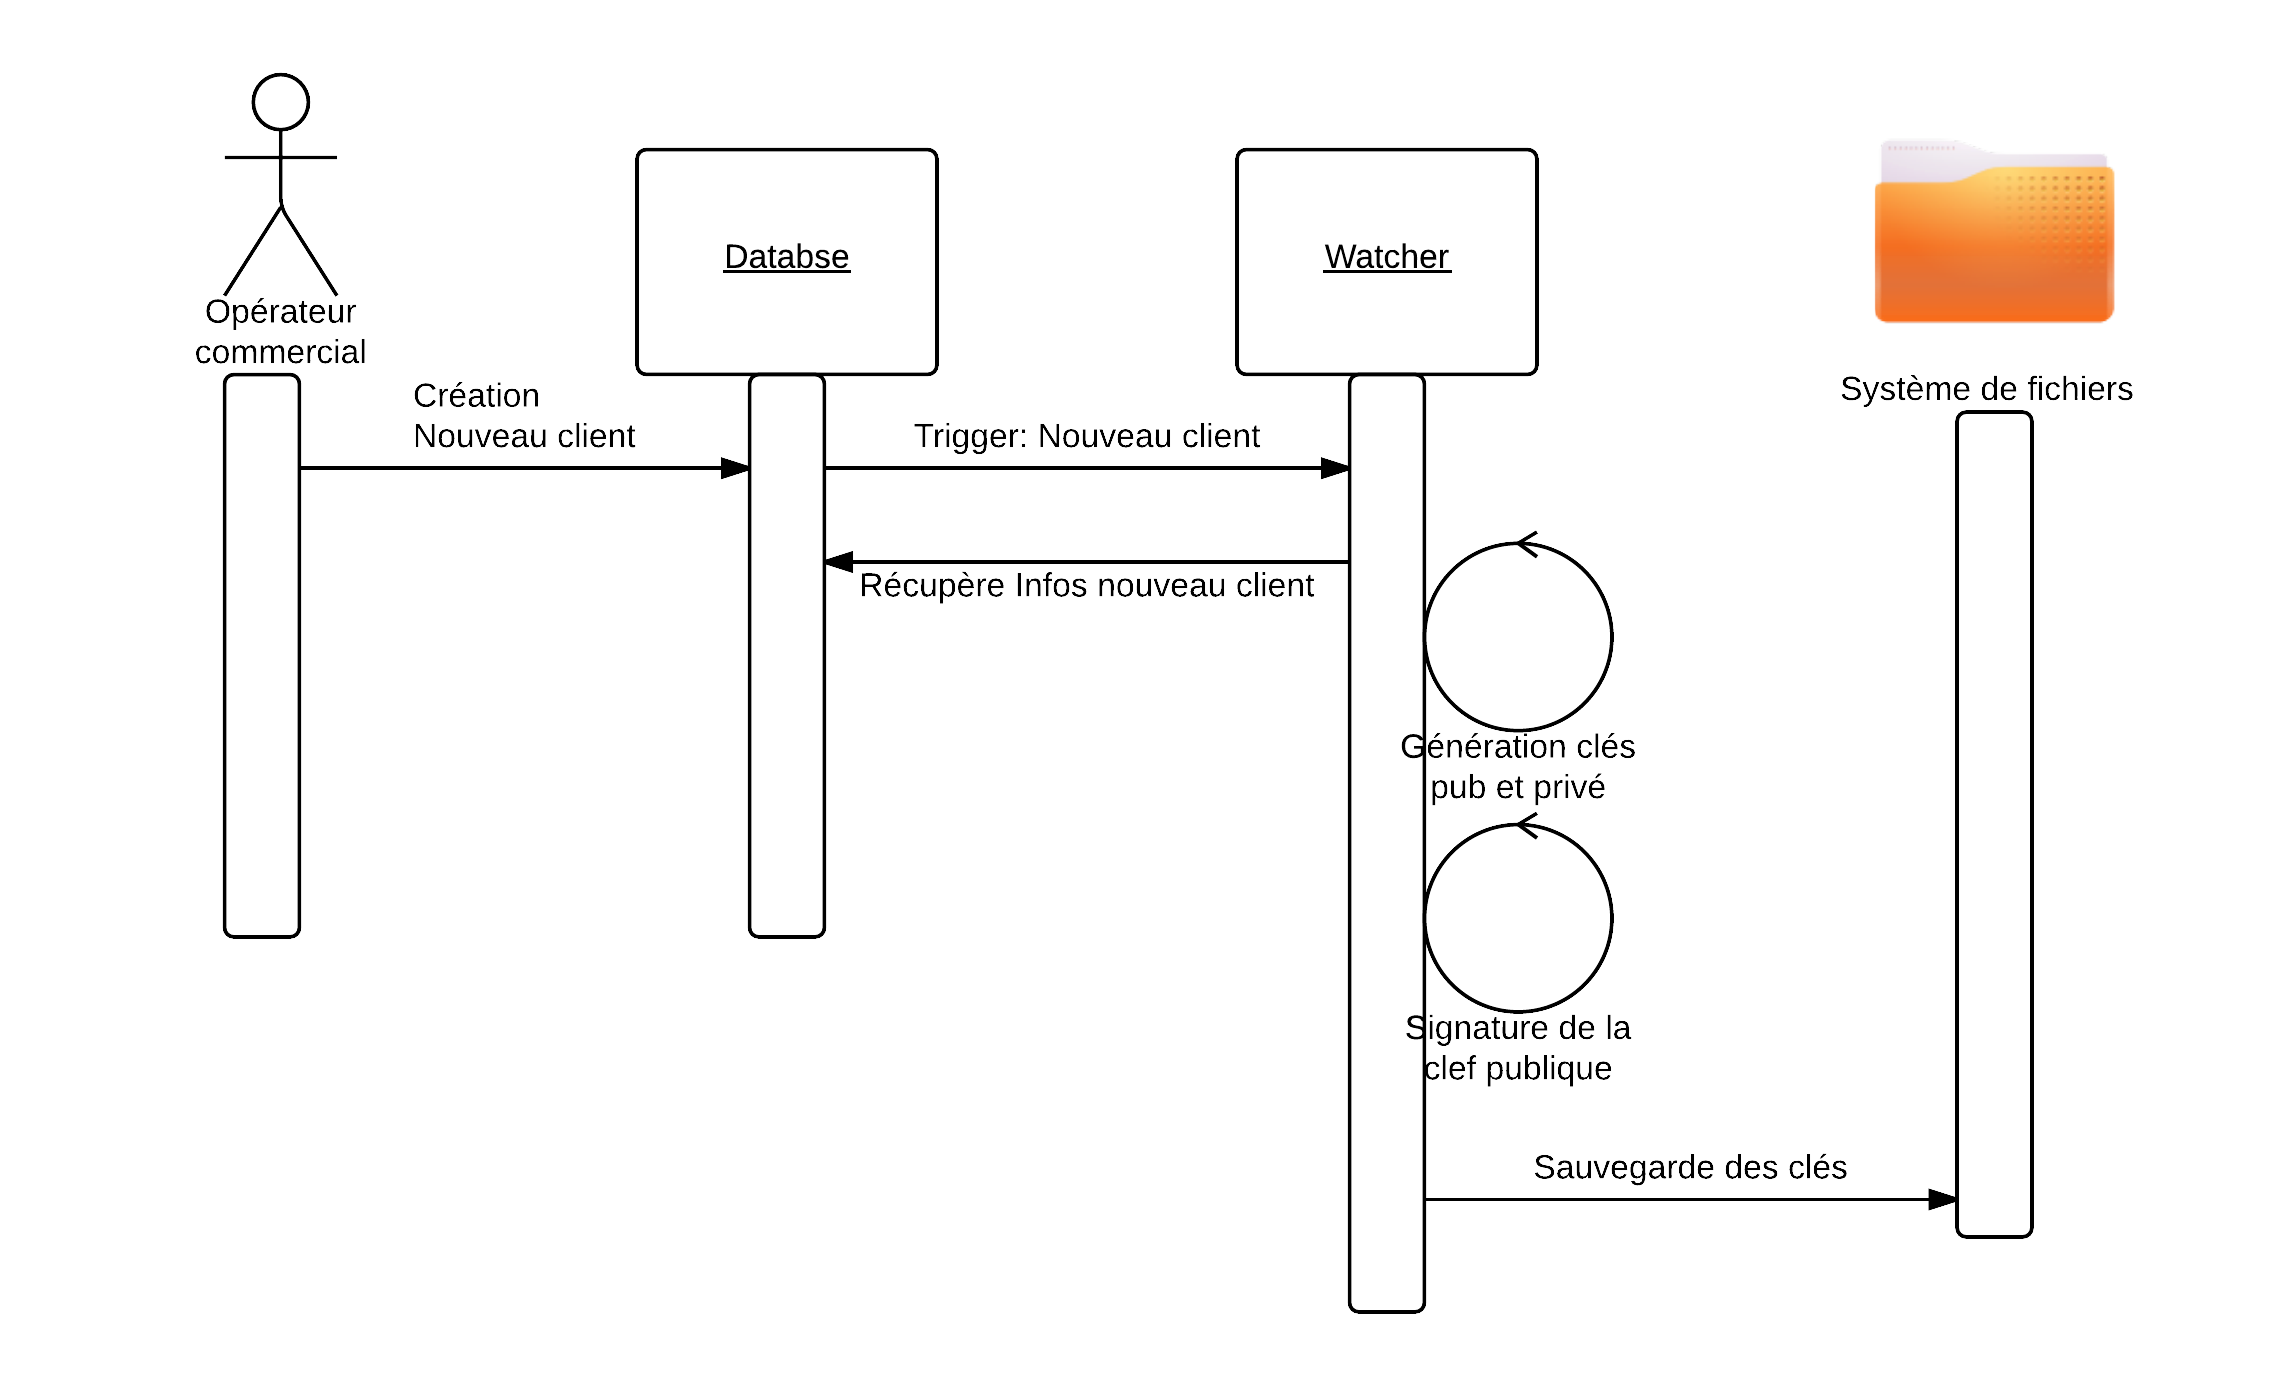
\includegraphics[scale=0.8]{images/new_client.png}
\label{fig:new_client}
\caption{Digramme de séquence: ajout d'un nouveau client}
\end{figure}

\begin{figure}
\centering
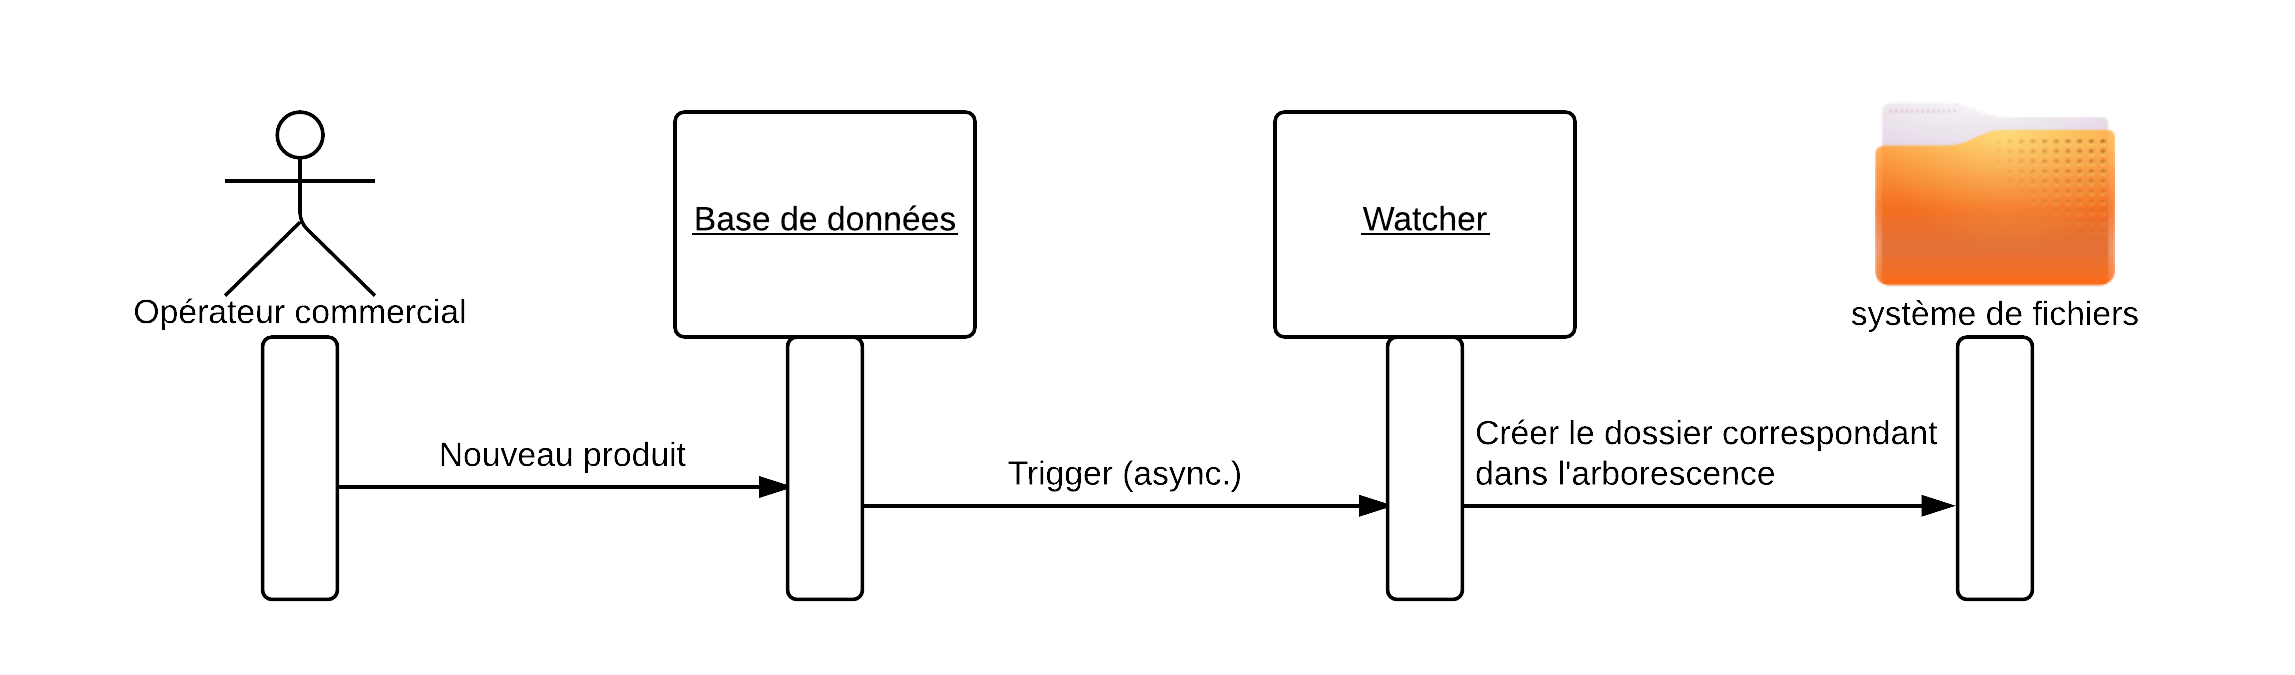
\includegraphics[scale=0.8]{images/new_product.png}
\label{fig:new_product}
\caption{Digramme de séquence: ajout d'un nouveau produit}
\end{figure}

\begin{figure}
\centering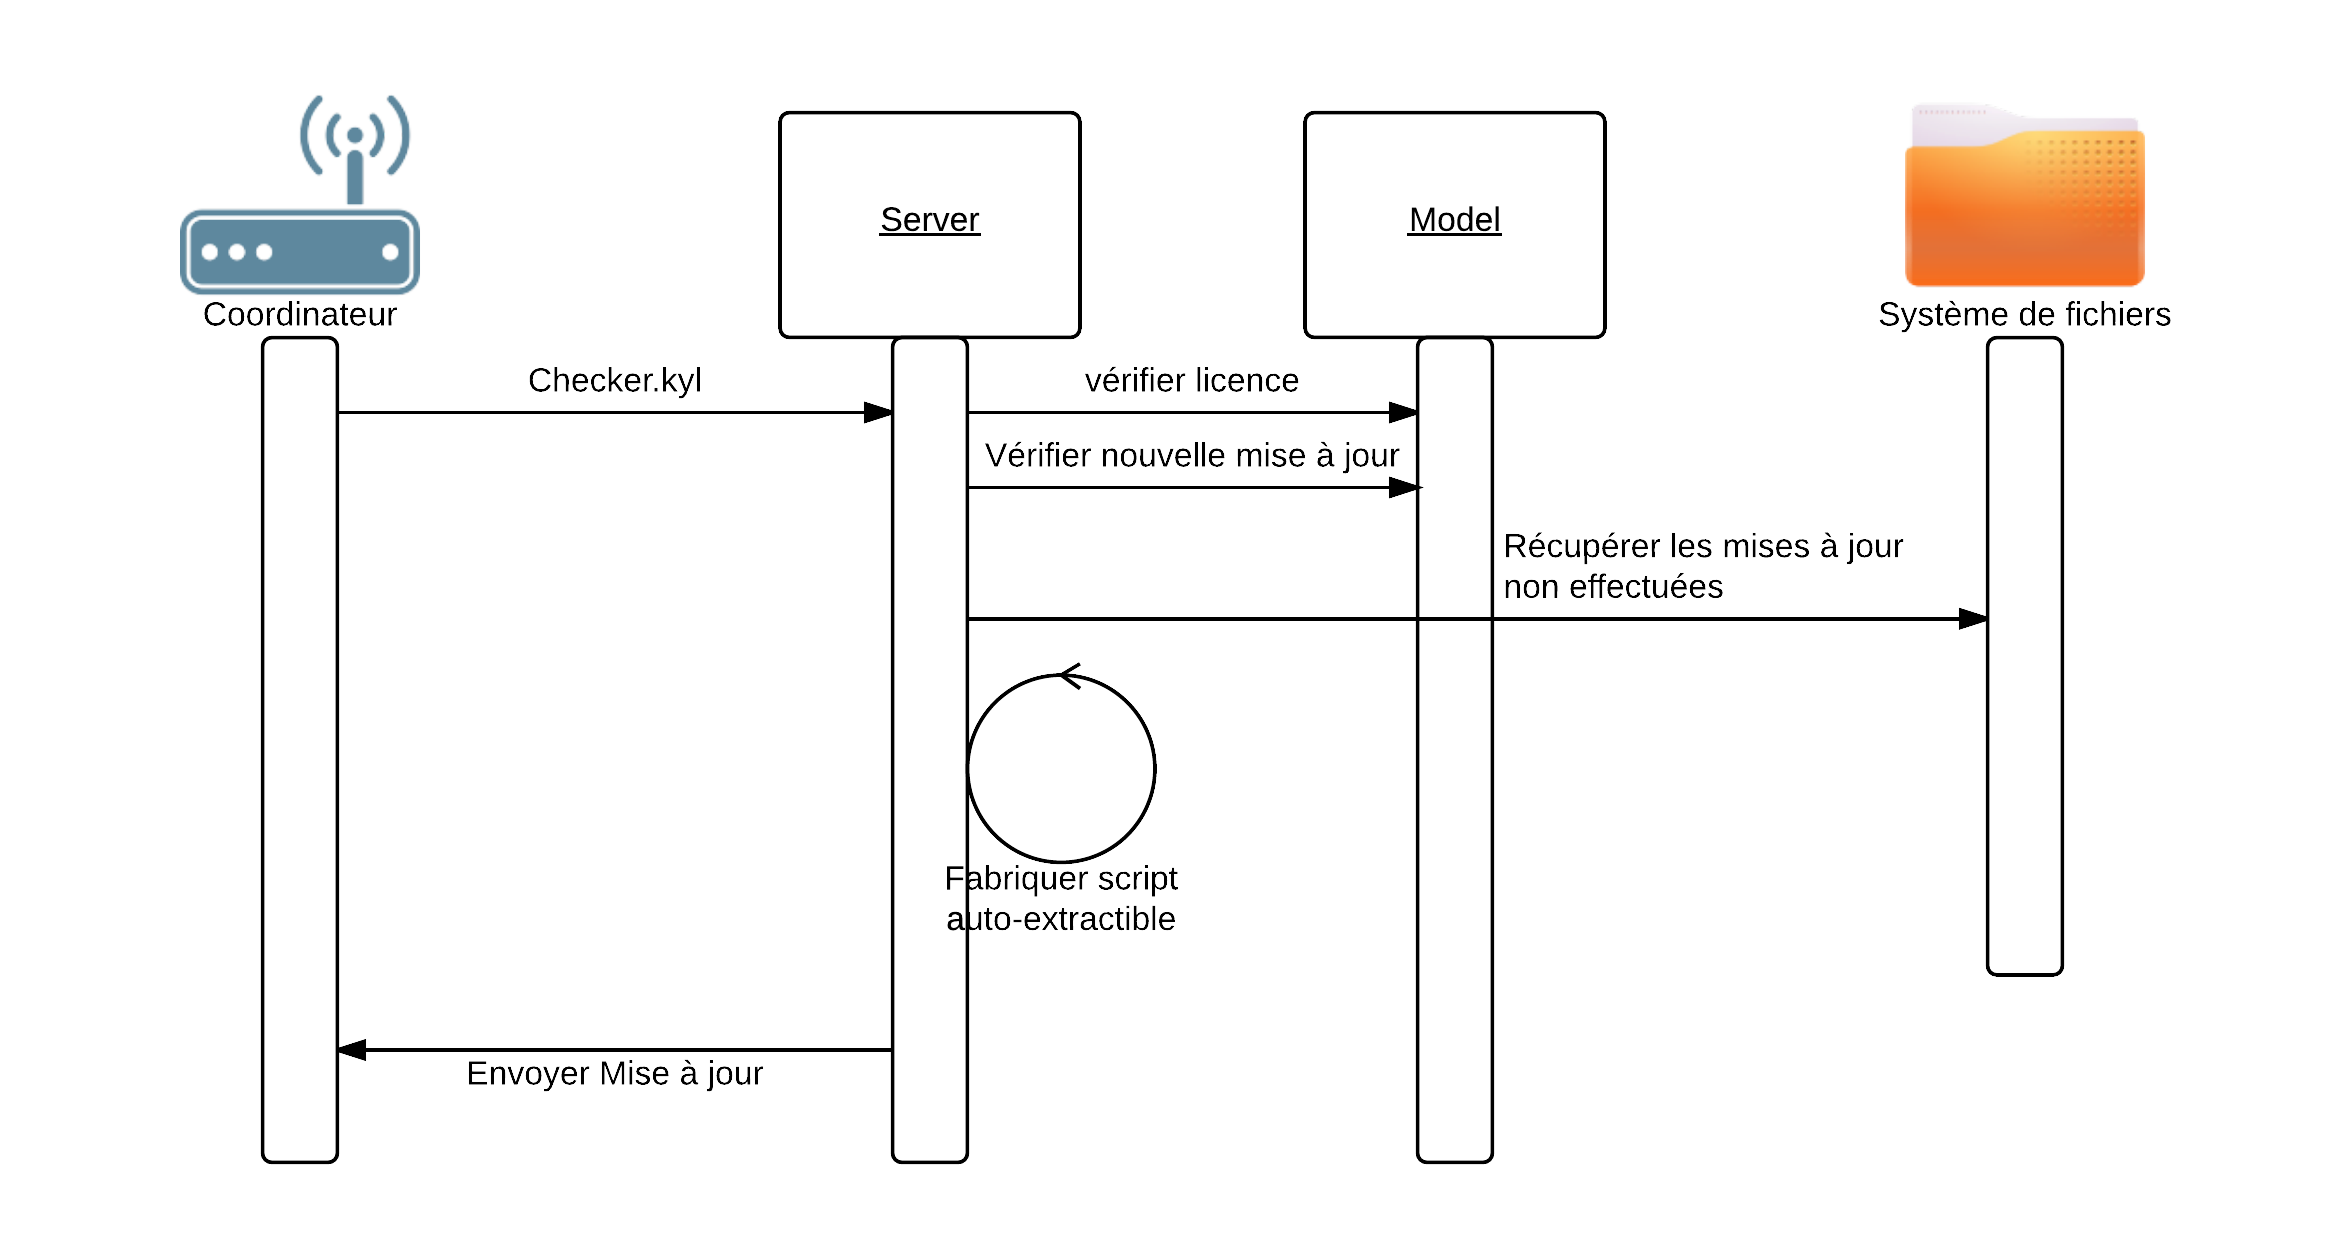
\includegraphics[scale=0.8]{images/maj.png}
\label{fig:maj}
\caption{Digramme de séquence: Mise à jour du coordianteur}
\end{figure}

\begin{figure}
\centering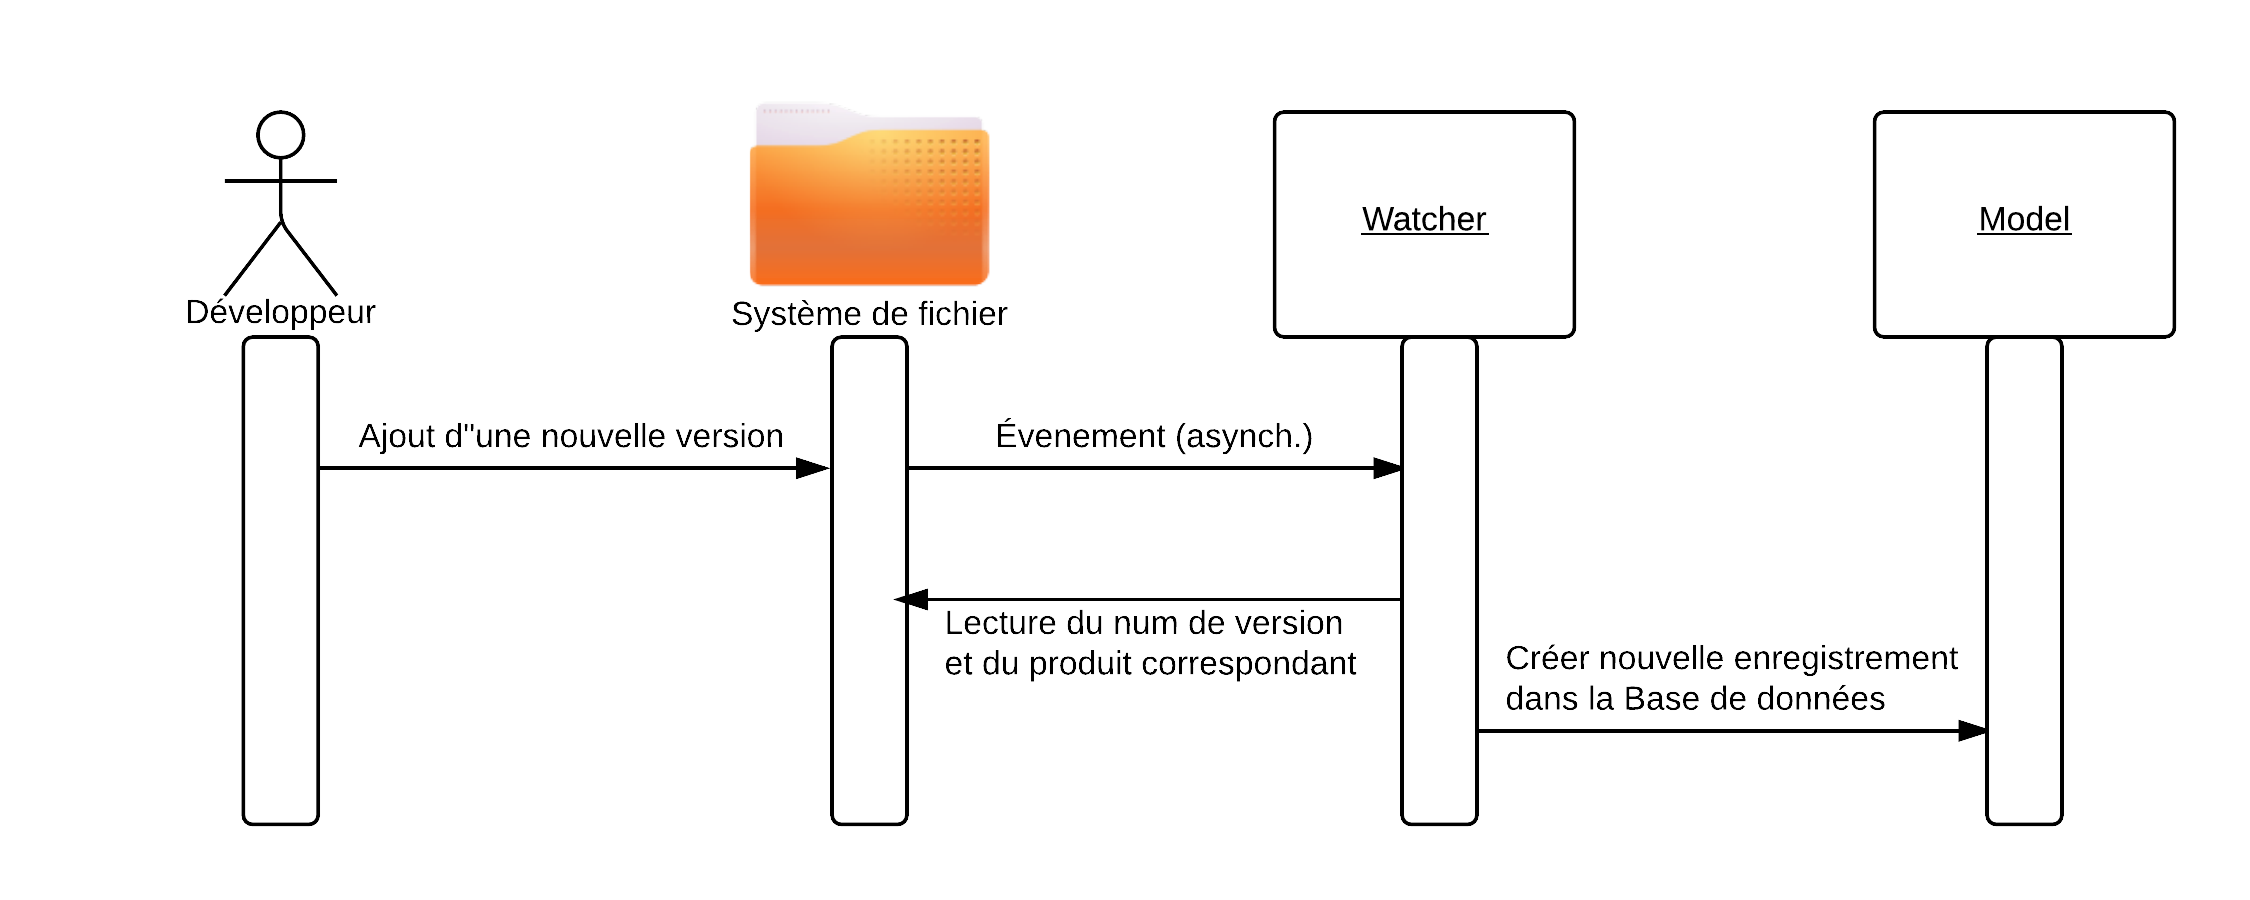
\includegraphics[scale=0.8]{images/seq_dev.png}
\label{fig:seq_dev}
\caption{Digramme de séquence: Ajout d'une nouvelle version dans le dépôt}
\end{figure}


\begin{comment}
\begin{itemize}
\item \texttt{themeensg.cls} : contient les personnalisations et macros utiles
\item \texttt{jury.tex} : pour la feuille de présentation du jury
\item le dossier \texttt{images} : il doit contenir toutes les images, il contient déjà le dossier logo avec celui de l'\ensg
\item \texttt{bibliographie.bib} contient la bibliographie
\end{itemize}
\end{comment}




\evenchapter[Mise en place et sécurisation d'une infrastructure virtuelle de production des logiciels:]{Mise en place et sécurisation d'une infrastructure virtuelle de production des logiciels:}

Le besoin se fait ressentir au sein de la société Kylia de disposer d'une infrastructure de production des logiciels lui permettant de gérer le patrimoine logiciel dont elle dispose et spécialement celui en relation avec le Géocube.  

\section{Système hôte:}

Pour déployer une infrastructure de production des logiciels. il faut disposer d'un serveur avec une adresse IP statique, permettant à tous les acteurs de centraliser leurs contributions et de les rendre accessibles aux autres en temps réel.

Selon la taille des entreprises et des performances demandées des solutions existent. Pour les PME (cas de la société Kylia) qui ne disposent pas moyens logistiques\footnote{installations électriques, systèmes de climatisation, connexion internet deterministique, ...} pour accueillir un serveur physique, Des prestataires, dont le métier est l'hébergement des data-centres proposent des solutions pour la location d'un serveur virtuel. Ainsi une société peut disposer d'un serveur hautement disponible sans pour autant l'accueillir physiquement.

Ce type de solution, communément connus sous le nom de VPS(Virtual Private Server), est accessible en ligne de commande à travers le protocole SSH (Shell sécurisé) et laisse la liberté complète à l'administrateur de gérer le système, comme dans un serveur physique.

Le prestataire selectionné garantit une accessibilité de 99.989\% ce qui correspond à 364.96 jours accessibles par an, une bande passante de 100Mbps, une puissance de calcul permettant de signer 114 certificats OpenSSL par seconde et par CPU.

Un tel serveur est adapté pour accueillir une infrastructure logicielle d'une PME ainsi que de proposer des services en ligne (voir chapitre3) pour un nombre de clients qu'on estime à vingts.

\subsection{Choix du système d'exploitation:}

Le système d'exploitation du VPS a été choisit en respectant les critères suivants:
\begin{itemize}
\item Grande communauté de développeurs et d'utilisateurs.
\item Stabilité.
\item Compatible avec le système d'exploitation sur lequel tourne le coordinateur(Debian) pour simplifier les tests.
\end{itemize}

Debian a été retenu comme système d'exploitation du VPS puisqu'il respecte tous ces points.

\section{Système de versioning:}
Un système de versioning sert principalement à:

\begin{itemize}
\item Garder des traces de toutes les modifications effectuées sur le code. et donc répondre aux question: qui a fait quoi et quand?
\item Coordonner le travail entre les développeurs.
\item disposer toujours de la dernière version pour effectuer les tests et déployer sur les serveurs de production.
\end{itemize}

Il existe deux principaux types de systèmes de versioning:
\begin{itemize}
\item Systèmes centralisés: Le dépôt central est hébérgé dans un serveur, tous les développeurs s'alignent sur la version du serveur et envoient leurs mdifications vers ce dépôt.
\item Systèmes décentralisés: chaque développeurs
\end{itemize}

Le contexte dans le quel s'inscrit le projet Géocube favorise le choix d'un système de versioning décentralisé garantissant à chacun des deux organisme intervenant sur le projet (l'IGN et Kylia) de disposer des versions complètes des logiciels en respectant les particularités que chaque organisme peut avoir.

Ainsi nous avons opté pour un système de versioning basé sur Git. Et ceci à travers Gitolite.

Gitolite est une réécriture de Gitosis, par Sitaram Chamarty. Il permet de gérer des dépôts Git à l'aide d'un.. dépôt Git, il attribut aux utilisateurs du système des droits spécifiques comme la lecture, écriture, etc. Il possède un fichier de configuration qui permet le contrôle d'accès sur chaque branche, incluant des spécifications comme qui peut ou ne peut pas revenir sur une branche donnée.

Gitolite utilise évidement les clés publiques ssh pour l'ajout d'utilisateur, mais il est intéressant car il interdit ses utilisateurs de se connecter au shell dans les dépôts. Ainsi aucune modification ne peut être effectuer sur le code d'un dépôt sans commiter les modifications sans C'est l'un des points importants de sécurité auxquels répond Gitolite.

 La configuration de Gitolite est simple. Un dépôt de configuration nommé gitolite-admin est créé sur le serveur, ainsi que son clône dans le répertoire personnel de l'administrateur. C'est dans celui-ci les dépôts sont configurés. Cette configuration comprend un fichier et un dossier :
\begin{itemize}
\item gitolite.conf : fichier de configuration de Gitolite, contenant les dépôts, leurs utilisateurs-groupes et leurs droits associés;
\item keydir : dossier contenant les clés publiques des utilisateurs autorisés, sous la forme user-name.pub.
\end{itemize}

La configuration de Gitolite utilisant un dépôt Git spécifique, il sera nécessaire de commiter les changements effectués pour qu'ils prennent effet.

Tous les codes de la société Kylia sont actuellement intégrés à l'outil de versionning. Une interface web permettant de superviser tous les dépôts a été créées à l'aide de Gitlist. Cette interface ne permet que la visualisation des commits, les branches, statistiques d'utilisation, ... aucune modification du code n'est permise à partir de cette interface.

\section{Gestionnaire de bugs:}
Un gestionnaire de bugs, et contrairement à ce que son nom peut laisse croire, ne sert pas qu'à gérer les bugs. C'est un système d'information qui permet de coordonner le travail du développeur, testeur et opérateur commercial. Ce système permet de reporter les bugs, les propositions d'amélioration, les remarques des clients ainsi que de suivre l'évolution de la réalisation et la réponse des développeurs à tout ça.

Le plus connu des gestionnaires de bugs est BugZilla, c'est une solution libre de la fondation Mozilla qui a su fédérer une grande communauté de développeurs et d'utilisateurs. C'est une solution stable qui est utilisée dans plusieurs grands projets informatiques\footnote{Le plus connu reste le navigateur FireFox}. Elle a donc été choisit comme gestionnaire de bugs au sein de la société Kylia. Le lecteur curieux désirant Son installation sur le serveur de production et sa configuration peut se reférer directement à sa documentation officielle.


%-------------------------------------------------------------------------------
\newevenpage
\chapter*{Conclusion}
  \addcontentsline{toc}{part}{Conclusion}
  \vspace{1.5cm}

Les développements nécessaires à l'implémentation de la solution NFC dans le Géocube était une réelle chance de travailler, pour la première fois, sur le noyau d'un système d'exploitation en temps-réel, de comprendre le fonctionnement de ses composants et de les manipuler. Cette partie du stage était une opportunité de s'ouvrir sur le monde de l'électronique, de comprendre de processus par lequel passe une carte électronique depuis sa conception jusqu'à sa fabrication et d'entreprendre, moi même, des tests et des expérimentations électroniques en vue de valider les hypothèses émises lors de la phase ...

La deuxième partie du stage relative au développement de Sharokey était pour moi une mise en pratique des connaissances que j'ai acquis durant mon année de spécialité à l'ENSG, de décomposer le système d'information en couches: de la partie matérielle jusqu'à l'interface homme-machine en passant par la sécurité du systèmes, le développements des composants, jusqu'aux tests et mise en production.

La troisième partie qui traite de la mise en place d'une infrastructure virtuelle de production des logicielles au sein de la société Kylia est une 

Enfin, durant ce stage j'ai aussi effectué un travail de réflexion autour d'un sujet de thèse proposé par LOEMI et Kylia et qui s'articule autour du système Géocube. Un projet de recherche a été produit, voir Annexe I.

%-------------------------------------------------------------------------------
\newevenpage
\chapter*{Bibliographie:}
  \addcontentsline{toc}{part}{Bibliographie}
  \vspace{1.5cm}

[1]Tanenbaum, Andrew (2008). Modern Operating Systems. Upper Saddle River, NJ: Pearson/Prentice Hall. p. 160. ISBN 978-0-13-600663-3.

[2]Ortiz, C. Enrique (June 2006). "An Introduction to Near-Field Communication and the Contactless Communication API".

[3]Electronista Article: New NFC spec lets two phones swap messages, October 2011

[4]"Android 4.1 APIs". Android Developer Network

[5]Charles A. Walton "Portable radio frequency emitting identifier" U.S. Patent 4,384,288 issue date May 17, 1983.

[6]ISO/IEC 14443-1:2008 Identification cards -- Contactless integrated circuit cards -- Proximity cards -- Part 1: Physical characteristics

[7]ISO/IEC 14443-2:2010 Identification cards -- Contactless integrated circuit cards -- Proximity cards -- Part 2: Radio frequency power and signal interface

[8]ISO/IEC 14443-3:2011 Identification cards -- Contactless integrated circuit cards -- Proximity cards -- Part 3: Initialization and anticollision

[9]ISO/IEC 14443-4:2008 Identification cards -- Contactless integrated circuit cards -- Proximity cards -- Part 4: Transmission protocol

[10]Menezes, Alfred; van Oorschot, Paul C.; Vanstone, Scott A. (October 1996). Handbook of Applied Cryptography. CRC Press. ISBN 0-8493-8523-7.

[11]Grime, James. "RSA Encryption". Numberphile. Brady Haran

[12]"Trust". Git Concepts. Git User's Manual. 2006-10-18




%-------------------------------------------------------------------------------
% Insertion de la bibliographie
\newevenpage
\nocite{*}
\bibliographystyle{apalike}
\bibliography{bibliographie.bib}

\newevenpage
\begin{appendices} 
\label{beginappendices}
\annexe[Projet de recherche]{Projet de recherche}
\label{annexekalman}
\section*{Titre:}
Utilisation de réseaux de capteurs pour la mesure conjointe des déformations du sol par GPS de précision et de paramètres physico-chimiques dans un contexte volcanique.
\section*{Contexte:}
La miniaturisation des capteurs ainsi que la baisse des coûts de fabrication et de la consommation électrique des puces GNSS sont des facteurs qui peuvent laisser à envisager d'abandonner sur le terrain un réseau de capteurs opérant en permanence. Certains de ces capteurs GNSS permettent d'effectuer des mesures sur la phase donnant la possibilité de remonter à des précisions millimétriques, d'où l'idée d'un réseau de Géocubes. Le système Géocube est un réseau de capteurs GPS conçu et développé par le Laboratoire d'Opto-Éléctronique de Mesure et d'Instrumentation de l'Institut Géographique et Forestière Nationale. Il a comme objectif de mesurer les déformations avec une précision millimétrique. Ce réseau de capteurs a la particularité d'être très peu gourmand en énergie. On peut envisager de l'abandonner dans un milieu difficilement accessible au moment de crises environnementales sans qu'on ait à se soucier de son alimentation continue en électricité. En plus d'un module radio, un Géocube peut supporter plusieurs couches de capteurs qui peuvent donner accès à des connaissances sur les caractéristiques physico-chimiques du milieu de déploiement. Un tel réseau peu opérer dans des milieux dangereux et difficilement accessibles, comme les volcans.

\section*{État de l'art:}

La surveillance instrumentale de l'activité volcanique est indispensable à la compréhension de ce phénomène géo-physique et à la prévision des éruptions. Aujourd'hui, Les volcans sont déjà surveillés par des réseaux de capteurs physico-chimiques, des stations GNSS permanentes et des méthodes de télédétection spatiale. Plusieurs méthodes existent et permettent d'avoir des précisions dépendantes du mode opératoire et la fréquence des mesures effectuées. Ces méthodes se basent principalement sur la détermination des variations des paramètres physico-chimiques lors d'une activité volcanique Géochimie, Magnétométrie, Micro-gravimétrie ou sur la mesure du mouvement de sol engendré par les variations ces mêmes activités Photogrammétrie, Géodésie spatiale, interférométrie Radar.

Un réseau de Géocubes permet de mesurer les déformations avec des précisions comparables à celles obtenues en utilisant les capteurs GNSS bi-fréquence avec la mesure de la phase en L2. Les tests effectués jusqu'à ce jour montrent qu'on peut atteindre une précision millimétrique en planimétrie et centimétrique en altimétrie sur un réseau sub-kilométrique.

Dans des milieux tectoniquement actifs et difficilement accessible, ce réseau de capteur peut s'avérer d'une importance cruciale. La précision spatio-temporelle qu'il offre peut être utilisée pour dater et localiser avec une grande précision des phénomènes géo-physiques et géo-chimiques à l'aide de couches de capteurs qu'on peut embarquer dans un Géocube. Son faible coût de fabrication peut laisser envisager de l'abandonner dans des zones à risques en le dottant d'une couche de capteurs adaptée.

\section*{Objectifs scientifiques et industriels:}

L'objectif scientifique d'étudier l'apport de la fusion de capteurs GNSS et des capteurs physico-chimiques dans un réseau de Géocubes à la connaissance du volcanisme, la prédiction des éruptions volcanique et à la restitution des déformations du sol et des variations des paramètres physico-chimiques dans un contexte de crise. La question qu'on peut se poser serait alors: y-a t'il des phénomènes physico-chimiques, mais aussi optiques, dans des endroits plus profonds du cratères volcaniques et qui aideront à quantifier et à prédire la durée d'une éruption volcanique, la quantité de laves qui sera éjectée et à mieux comprendre la structure des gazes et des roches volcaniques?

La méthode proposée est une méthode instrumentale de surveillance volcanique en champ proche, dans un contexte de crise, basée sur la fusion des capteurs physico-chimiques et des capteurs GNSS. Cette méthode se basera essentiellement sur la mesure conjointe des variations des paramètres physico-chimiques et des variations surfaciques qui occurrent dans un contexte volcanique difficilement accessible par les humains et les machines de grande taille. En plus de l'apport que les systèmes GNSS peuvent avoir sur la localisation et la datation précises de ces phénomènes, ces systèmes peuvent mesurer avec une précision millimétrique les déformations surfaciques sur des grandes échelles de temps. Une combinaison de tous ces aspects pourrait alors donner naissance à un système de surveillance volcanique en champs proche, opérant parallèlement aux instruments de surveillance volcanique classiques, facilement déployable en temps de crise et capable d'aller opérer dans des endroits difficilement accessibles, facilitant ainsi la prédiction des éruptions et la génération d'alertes.

La miniaturisation des capteurs, l'autonomie des réseaux Géocubes sont des facteurs clés qui peuvent laisser envisager, en cas de validation scientifique de la méthode proposée, d'industrialiser des versions de Géocubes dotées de capteurs permettant mieux connaître l'environnement de déploiement, assez robuste pour supporter les conditions extrêmes d'un contexte de crise (robustesse mécanique, température opérationnelle élevée, ...) , et d'apporter ainsi des dimensions d'analyse en plus de la dimension spatiale disponible dans la version actuelle. Ce système de surveillance viendra se superposer aux méthodes existantes de surveillance volcanique, et apportera des connaissances additionnelles (Exemple: utiliser un réseau de Géocube dense pour fournir des points d'appui au sol aux méthodes de photogrammétrie spatiale. Comme le projet SVOBS2015.svobs.eu , ...).

\section*{Verrous scientifiques et techniques:}

Au fur et à mesure de l'avancement des travaux, plusieurs verrous scientifiques et techniques devront être levés. La principale problématique concerne la taille des réseaux des Géocubes, les tests effectués jusqu'à ce jour ont donné des précisions raisonnables dans des réseaux de taille sub-kilométrique. Une amélioration de la méthode de résolution des ambiguïtés atmosphériques actuellement implémentée est à prévoir pour pouvoir couvrir des surfaces plus importantes, adaptées à un contexte volcanique. Cette méthode de résolution des ambiguïtés atmosphériques nécessite aussi plusieurs heures de calculs pour obtenir une bonne précision, l'amélioration de cette méthode est essentielle si on compte déployer un réseau de Géocubes en contexte de crise, là ou chaque minute est importante et cruciale. S'ajoute à cela plusieurs verrous technologiques liés à la gestion de la consommation électrique dans des endroits ou l'énergie solaire serait insuffisante pour couvrir le besoin d'un Géocube en énergie. Des stratégies de gestion énergétique seraient alors à définir et à implémenter pour garantir une plus longue durée opérationnelle dans un contexte de crise. La robustesse du Géocube (mécanique et thermique) est un point important si on prévoit de le larguer par drone. Une stratégie de déploiement est aussi à définir et la faisabilité technique d'un déploiement par drones est à démontrer.

\section*{Méthodologie de recherche:}

Ce projet de recherche se trouve dans l'intersection de plusieurs sciences et disciplines Géophysique, Géochimie, Informatique et systèmes embarqués, Analyse de données. La méthodologie de recherche proposée pour ce projet est une méthodologie de recherche expérimentale et observationnelle qui passe par les étapes conventionnelles de la méthode scientifique: Question générale, affinage, conception de l'expérimentation, observation, analyse, conclusion et publication. Tout d'abord, Un dégrossissage et une décomposition du sujet en plusieurs hypothèses basées sur les observations effectuées devra être réalisé. Un affinage de ces hypothèses basé sur les résultats obtenus lors des expériences sur le terrain. Une analyse des données s'en suivra pour tirer les conclusions et les enseignements nécessaires à la réitération de ce processus.

\section*{Planning des travaux}

Le planning des travaux prévoit deux expériences sur le terrain. La première à réaliser en première année de thèse, nécessitera le développement d'une couche de capteurs géophysiques, et électrochimiques. Les données issues de cette expérience seront traitées et analysées pour tirer les conclusions nécessaires à la conception de la deuxième expérience qui se tiendra en deuxième année de thèse. Cette deuxième et dernière expérience a pour but de valider les enseignements tirés de la première expérience, d'affiner la liste des capteurs utilisés dans le Géocube, et de tirer les conclusions scientifiques nécessaires à la validation de la méthode de surveillance en question.



\end{appendices} 

\end{document}